\documentclass{article}

%\usepackage{fullpage}
\usepackage{amsmath,amssymb,amsfonts,amsthm,stmaryrd}
%\usepackage{stmaryrd}

\usepackage{mathpazo} % math & rm
\linespread{1.05}        % Palatino needs more leading (space between lines)
\usepackage[scaled]{helvet} % ss
\usepackage{courier} % tt
\normalfont
\usepackage[T1]{fontenc}

\usepackage{tikz-cd}

\usepackage{todonotes}
\usepackage{lscape}
\usepackage{rotating}

\usepackage{cleveref}

\newcommand{\Z}{\mathbb Z}
\renewcommand{\S}{\mathbb S}
\newcommand{\F}{\mathbb F}
\newcommand{\G}{\widehat{\mathbb G}}
\newcommand{\R}{\mathbb R}
\newcommand{\RP}{\R\mathrm P}
\newcommand{\C}{\mathbb{C}}
\newcommand{\CP}{\C\mathrm P}
\newcommand{\A}{\widehat{\mathbb{A}}}
\newcommand{\Q}{\mathbb{Q}}
\newcommand{\M}{\mathcal{M}}
\newcommand{\FH}{\textbf{FH}}
\newcommand{\CH}{\textbf{CH}}
\renewcommand{\L}{\mathcal{L}}
\renewcommand{\H}{\mathcal{H}}
\renewcommand{\P}{\mathbb{P}}
\newcommand{\W}{\mathbb W}
\newcommand{\m}{m}

\newcommand{\<}{\langle}
\renewcommand{\>}{\rangle}
\newcommand{\sm}{\wedge}
\newcommand{\Susp}{\Sigma}
\renewcommand{\phi}{\varphi}
\renewcommand{\epsilon}{\varepsilon}
\newcommand{\eps}{\varepsilon}
\newcommand{\mmod}{/\!\!/}
\newcommand{\co}{\colon\thinspace}
\newcommand{\into}{\hookrightarrow}
\newcommand{\cotensor}{\square}
\renewcommand{\th}{\textsuperscript{th}}

\newcommand{\context}[1]{\mathcal{M}_{#1}}
\newcommand{\CatOf}[1]{\mathsf{#1}}
\newcommand{\ps}[1]{\llbracket{#1}\rrbracket}
\newcommand{\moduli}[1]{\mathcal{M}_{\mathbf{#1}}}
\newcommand{\OS}[2]{\smash{\underline{#1}}_{#2}}
\newcommand{\sheaf}[1]{\mathcal{#1}}

\newcommand{\Spin}{\mathit{Spin}}
\newcommand{\String}{\mathit{String}}
\newcommand{\TMF}{\mathit{TMF}}
\newcommand{\tmf}{\mathit{tmf}}
\newcommand{\BP}{\mathit{BP}}
\newcommand{\MU}{\mathit{MU}}
\newcommand{\Tate}{\mathrm{Tate}}
\newcommand{\gl}{\mathit{gl}}
\newcommand{\GL}{\mathit{GL}}
\newcommand{\perf}{\mathrm{perf}}
\newcommand{\gpd}{\mathrm{gpd}}
\newcommand{\id}{\mathrm{id}}

\DeclareMathOperator{\Spec}{Spec}
\DeclareMathOperator{\Spf}{Spf}
\DeclareMathOperator{\Sch}{Sch}
\DeclareMathOperator{\colim}{colim}
\DeclareMathOperator{\End}{End}
\DeclareMathOperator{\Div}{Div}
\DeclareMathOperator{\SDiv}{SDiv}
\DeclareMathOperator{\Sq}{Sq}
\DeclareMathOperator{\Sym}{Sym}
\DeclareMathOperator{\Aut}{Aut}
\DeclareMathOperator{\Def}{Def}
\DeclareMathOperator{\Pic}{Pic}
\DeclareMathOperator{\Ext}{Ext}
\DeclareMathOperator{\hAut}{hAut}
\DeclareMathOperator{\Coord}{Coord}

\numberwithin{equation}{section}

\theoremstyle{plain}
\newtheorem{theorem}[equation]{Theorem}
\newtheorem{proposition}[equation]{Proposition}
\newtheorem{lemma}[equation]{Lemma}
\newtheorem{corollary}[equation]{Corollary}
\newtheorem{conjecture}[equation]{Conjecture}
\theoremstyle{definition}
\newtheorem{definition}[equation]{Definition}
\newtheorem{construction}[equation]{Construction}
\newtheorem{warning}[equation]{Important Warning}
\theoremstyle{remark}
\newtheorem{remark}[equation]{Remark}
\newtheorem{example}[equation]{Example}

\title{Formal Geometry in Algebraic Topology}
\author{Eric Peterson}

\begin{document}

\maketitle

\textbf{Class information}

\vspace{2\baselineskip} \noindent \textit{Meeting times: }
Spring 2016, MWF 12pm--1pm.

\vspace{2\baselineskip} \noindent \textit{Goals: }
The primary goal of this class is to teach students to view results in algebraic topology through the lens of (formal) algebraic geometry.

\vspace{2\baselineskip} \noindent \textit{Grading: }
This class won't have any official assignments. I'll give references as readings for those who would like a deeper understanding, though I'll do my best to ensure that no extra reading is required to follow the arc of the class.

I do want to assemble course notes from this class, but it's unlikely that I will have time to type \emph{all} of them up. Instead, I would like to ``crowdsource'' this somewhat: I'll type up skeletal notes for each lecture, and then we as a class will try to flesh them out as the semester progresses. As incentive to help, those who contribute to the document will have their name included in the acknowledgements, and those who contribute \emph{substantially} will have their name added as a coauthor. Everyone could use more CV items.



\newpage

\tableofcontents

\newpage

\section{Jan 25: Introduction}

The goal of this class is to communicate a certain \textit{weltanschauung} uncovered in pieces by many different people working in bordism theory, and the goal just for today is to tell a story about one theorem where it is especially apparent.

To begin, recall that a bordism theory $MX$, where $X$ is some suitable family of structure groups $X_n \to O(n)$, is a homology theory similar to singular homology but where the chains are constructed from $X$--structured manifolds and their boundaries.  The coefficient ring of $MX$, or its value $MX_*(*)$ on a point, gives the ring of $X$--bordism classes, and generally $MX_*(Y)$ of some space $Y$ gives a kind of ``bordism in families''.  There are evident comparison morphisms for the most ordinary kinds of bordism, given by replacing a chain of manifolds with an equivalent simplicial chain: \[MO \to H\Z/2, \quad MSO \to H\Z.\] In both cases, we can evaluate on a point to get ring maps $MO_*(*) \to \Z/2$ and $MSO_*(*) \to \Z$, called ``genera'' --- neither of which is very interesting, since they're both zero in positive degrees.\todo{A comparison of this with the usual spectrum definition of $MX$ appears in Switzer 12.35.}

However, having maps of homology theories (rather than just maps of coefficient rings) is considerably more data: we can extact from this a theory of integration.  Consider the following:
\begin{align*}
MSO_n K(\Z, n) & = \left\{ \text{oriented $n$--manifolds mapping to $K(\Z, n)$} \right\} / \sim \\
& = \left\{ \begin{array}{c}\text{oriented $n$--manifolds $M$} \\ \text{with a specified class $\omega \in H^n(M; \Z)$} \end{array}\right\} / \sim.
\end{align*}
The yoga of stable homotopy theory then allows us to build a composite \[\S^0 \xrightarrow{(M, \omega)} MSO \sm (\S^{-n} \sm \Susp^\infty_+ K(\Z, n)) \to MSO \sm H\Z \xrightarrow{\phi \sm 1} H\Z \sm H\Z \xrightarrow\mu H\Z,\] where $\phi$ is the orientation map, and this gives us an integer. This integer is $\int_M \omega$, and it comes equipped with a Stokes' theorem due to the relation ``$\sim$'', and we can begin to see what the techniques of stable homotopy theory have to offer.

Now take $X = e$ to be the trivial structure group, so that the Pontryagin--Thom construction gives an equivalence $Me \xrightarrow{\simeq} \S$.  It is thus possible (and some people have indeed taken up this viewpoint) that stable homotopy theory can be done solely through the lens of ``framed bordism''. I'm a stable homotopy theorist rather than a differential topologist, and so I prefer to view this the other way: the sphere spectrum $\S$ often appears in my life as a natural object, and I will sometimes replace it by $Me$, the framed bordism spectrum.  For example, often I encounter a ring spectrum $E$, and it comes equipped with a unit map $\S \to E$, which I can reconsider as a ring map $\S = Me \to E$.  Following along the lines of the previous paragraph, we learn that we can thus think of any ring spectrum $E$ as automatically equipped with a theory of integration for framed manifolds.

Sometimes, as in the examples above, this unit map factors: \[\S = Me \to MO \to H\Z/2.\]  This is a witness to the overdeterminacy of $H\Z/2$'s integral for framed bordism: if the framed manifold is pushed all the way down to an unoriented manifold, there is still enough residual data to define the integral.  For a generic ring spectrum $E$, we can ask the analogous question: for a Hausdorff filtration on $O$ by structure groups, what stage does the unit map $Me \to E$ factor through?  The map $SO \to O$ considered above is the beginning of the Postnikov filtration of $O$, and we include a diagram of this filtration and some interesting integration theories related to it:
\begin{center}
\begin{tikzcd}
Me \arrow{r} \arrow{rrd} \arrow{rrrd} \arrow{rrrrd} & \cdots \arrow{r} & M\Spin \arrow{r} \arrow[crossing over]{d} & MSO \arrow{r} \arrow[crossing over]{d} & MO \arrow[crossing over]{d} \\
& & ko & H\Z & H\Z/2.
\end{tikzcd}
\end{center}

This is the situation homotopy theorists found themselves in some decades ago, in the wake of two important results of Ochanine and Witten. Ochanine had proven the following mysterious theorem using analytic techniques:

\begin{theorem}[Ochanine]
There is a cobordism invariant $o(M)$ of an oriented manifold $M$ which is a level $2$ modular form. It is somewhat multiplicative: if $F \to E \to M$ is an exceedingly nice fibration, then $o(E) = o(F) \cdot o(M)$.
\end{theorem}

\noindent Witten then strengthened this result considerably:

\begin{theorem}[Witten]
Ochanine's genus is in fact multiplicative. Also, if $M$ is a Spin manifold such that twice its first Pontryagin class vanishes, then $o(M)$ can be ``refined''\todo{What does ``refined'' mean, anyway? It's a square root, maybe?} to a level $1$ modular form $w(M)$.
\end{theorem}

\noindent However, neither party gave indication that their result should be valid ``in families'', and no theory of integration was produced.  It wasn't even clear what such a claim would mean: to give a topological enrichment of these theorems would mean finding a ring spectrum $E$ such that $E_*(*)$ had something to do with modular forms.  Around the same time, Landweber, Ravenel, and Stong began studying ``elliptic cohomology'' for independent reasons, and a decade later Ando, Hopkins, and Strickland put them together in the following theorem:

\begin{theorem}[Ando--Hopkins--Strickland]
If $E$ is an ``elliptic cohomology theory'', then there is a canonical map $M\String \to E$ called the $\sigma$--orientation.  Specializing to Tate $K$--theory $K^{\Tate}$, the induced map $M\String_* \to K^{\Tate}_*$ is Witten's genus.
\end{theorem}

We now come to the motivation for this class.  The homotopical $\sigma$--orientation was actually first constructed using formal geometry.  The original proof of Ando--Hopkins--Strickland begins with a reduction to understanding maps \[MU[6, \infty) \to E,\] and then they work to show that they can complete the missing arrow in the diagram
\begin{center}
\begin{tikzcd}
MU[6, \infty) \arrow{r} \arrow{rd} & M\String \arrow[densely dotted]{d} \\
& E.
\end{tikzcd}
\end{center}
Leaving aside the extension problem for the moment, their main theorem is the following description of the cohomology ring $E^* MU[6, \infty)$:
\begin{theorem}[Ando--Hopkins--Strickland]
For $E$ an even--periodic cohomology theory, \[\Spec E_* MU[6, \infty) \cong C^3(\G_E; \sheaf I(0)),\] where ``$C^3(\G_E; \sheaf I(0))$'' is a certain scheme.  When $E$ is taken to be elliptic, so that there is a specified isomorphism $\G_E \cong C^\wedge_0$ for $C$ an elliptic curve, this furnishes the scheme with a canonical point. Hence, there is a preferred class $MU[6, \infty) \to E$, natural in the choice of elliptic $E$.
\end{theorem}

\noindent Our real goal is to understand theorems like these.  The structure of the class will be, more or less, to work through a sequence of case studies where this perspective on algebraic topology shines through most brightly.  We'll start by working through Thom's calculation of the homotopy of $MO$, which simultaneously holds the attractive features of being free of technical complexity while revealing essentially all of the structural complexity.  Having seen that through to the end, we'll then work on reinforcing our technical underpinnings, and then we'll venture on to other examples.  The overriding theme of the class will be that this is a good organizing principle that gives us one avenue of insight into how homotopy theory functions. 




\section{Jan 27: Thom spectra and the Thom isomorphism}

Our first case study is a sequence of theorems about the unoriented bordism spectrum $MO$.  I wanted to begin by recalling one definition of the spectrum $MO$, since it will be useful to us throughout the semester.

\begin{definition}
For a spherical bundle $S^{n-1} \to \xi \to X$, its Thom space is given by the cofiber \[\xi \to X \xrightarrow{\text{cofiber}} T(\xi).\]
\end{definition}
\begin{proof}[``Proof'' of definition]
There's a more usual construction of the Thom space too: the associated disk bundle by gluing an $n$--disk in fiberwise, then taking the one--point compactification: \[T(\xi) = (\xi \sqcup'_{S^{n-1}} D^n)^+.\] How does this compare? Well, the thickening of $\xi$ is an $n$--disk bundle is the same thing as taking the mapping cylinder on $\xi \to X$. Since the inclusion into the mapping cylinder is now a cofibration, the quotient by this subspace agrees with both the cofiber of the map and the one--point compactification.
\end{proof}

Before proceeding, here are two important examples:
\begin{example}\label{TrivialBundleThomExample}
If $\xi = S^{n-1} \times X$ is the trivial bundle, then $T(\xi) = S^n \sm (X_+)$.  This is supposed to indicate what Thom spaces are ``doing'': if you feed in the trivial bundle then you get the suspension out, so if you feed in a twisted bundle you should think of it as a \textit{twisted suspension}.
\end{example}

\begin{example}\label{RPnThomExample}
Let $\xi$ be the tautological $S^0$--bundle over $\RP^\infty = BO(1)$.  Because $\xi$ has contractible total space, the cofiber degenerates and it follows that $T(\xi) = \RP^\infty$. More generally, arguing by cells shows that the Thom space for the tautological bundle over $\RP^n$ is $\RP^{n+1}$.
\end{example}

Now we catalog a bunch of useful properties of the Thom space functor. Firstly, recall that a spherical bundle over $X$ is the same data as a map $X \to B \GL_1 S^{n-1}$, where $\GL_1 S^{n-1}$ is the subspace of $F(S^{n-1}, S^{n-1})$ expressed by the pullback
\begin{center}
\begin{tikzcd}
\GL_1 S^{n-1} \arrow{r} \arrow{d} & F(S^{n-1}, S^{n-1}) \arrow{d} \\
\Aut_{h\CatOf{Spaces}} S^{n-1} \arrow{r} & \End_{h\CatOf{Spaces}} S^{n-1} \arrow[-,double]{r} & \pi_0 F(S^{n-1}, S^{n-1}).
\end{tikzcd}
\end{center}
We can interpret $T$ as a functor from the slice category over $BGL_1 S^{n-1}$ to $\CatOf{Spaces}$: maps \[Y \xrightarrow{f} X \xrightarrow{\xi} B \GL_1 S^{n-1}\] induce maps $T(f^* \xi) \to T(\xi)$, and $T$ is suitably homotopy-invariant.

Next, a common source of spherical bundles is taking the spherical subbundle of a vector bundle.  Since rank $n$ vector bundles are also classified by an object $BO(n)$, this begets a map $J_{\R}^n: BO(n) \to B \GL_1 S^{n-1}$ for each $n$.  Homotopy theorists are very interested in the block--inclusion maps $i^n: BO(n) \to BO(n+1)$ and the colimit $BO = BO(\infty)$.  The suspension functor induces a map $\GL_1 S^{n-1} \to \GL_1 S^n$, and we are led to ask about the compatibility of these operations.  As a route to answering this, the block--inclusion maps are a special case of a more general direct sum map $\oplus: BO(n) \times BO(m) \to BO(n+m)$, given by the precomposition \[BO(n) = BO(n) \times * \xrightarrow{\operatorname{id} \times \text{triv}} BO(n) \times BO(1) \xrightarrow\oplus BO(n+1).\] The spaces $B \GL_1 S^{n-1}$ enjoy a similar ``collective monoid'' structure, given by taking the fiberwise join two spherical bundles with a common base.
\begin{lemma}
The fiberwise join is represented by maps \[B\GL_1 S^{n-1} \times B\GL_1 S^{m-1} \to B\GL_1 S^{n+m-1},\] and these maps commute with the block sum maps on the $BO(n)$ family. \qed
\end{lemma}
\noindent Again taking a cue from $K$--theory, we take the colimit as $n$ grows large.
\begin{corollary}
There is a map of $H$--spaces $J_{\R}: BO \to B\GL_1 \S$ called the \textit{stable $J$--homomorphism}. \qed
\end{corollary}
\noindent Finally, we can ask about the compatibility of $T$ with all of this:
\begin{lemma}
$T$ is monoidal: it carries fiberwise joins to smash products of spaces. \qed
\end{lemma}

We are now prepared to define our spectrum $MO$.  The unstable $J$--maps $J_{\R}^n: BO(n) \to B\GL_1 S^{n-1}$ give Thom spaces $T(J_{\R}^n)$,\todo{Be careful about dimension here: you really mean a reduced tautological bundle, related to how $BO$ has only one connected component.} equipped with maps\todo{Fix this equation.} \[\Susp T(J_{\R}^n) = T(J_{\R}^n \oplus \text{triv}) \to T(J_{\R}^{n+1}).\] Setting $MO(n) = \Susp^{-n} \Susp^\infty T(J_{\R}^n)$, we again assemble this data into a single object: \[MO := \colim_n MO(n) = \colim_n \Susp^{-n} T(J_{\R}^n).\]

The spectrum $MO$ has several remarkable properties.  The most basic such property is that it is a ring spectrum, and this follows immediately from $J_{\R}$ being a homomorphism of $H$--spaces.  Much more excitingly, we can also deduce the presence of Thom isomorphisms just from the properties stated thus far.  That $J_{\R}$ is a homomorphism means that the following square commutes:
\begin{center}
\begin{tikzcd}
BO \times BO \arrow{r}{\sigma, \simeq} \arrow[bend right]{rrd} & BO \times BO \arrow{r}{\mu} \arrow{d}{J_{\R} \times J_{\R}} & BO \arrow{d}{J_{\R}} \\
& B\GL_1 \S \times B\GL_1 \S \arrow{r}{\mu} & B\GL_1 \S.
\end{tikzcd}
\end{center}
We have extended this square very slightly by a certain shearing map $\sigma$ defined by $\sigma(x, y) = (xy^{-1}, y)$.\todo{$\sigma$ \emph{almost} shows up in giving a categorical definition of a $G$--torsor.  I wish I understood this, but I always get tangled up.}  It's evident that $\sigma$ is a homotopy equivalence, since just as we can de-scale the first coordinate by $y$ we can re-scale by it.  We can calculate directly the behavior of the long composite: \[J_{\R} \circ \mu \circ \sigma(x, y) = J_{\R} \circ \mu(xy^{-1}, y) = J_{\R}(xy^{-1}y) = J_{\R}(x).\]  It follows that the second coordinate plays no role, and that the bundle classified by the long composite can be written as $J_{\R} \times 0$.\footnote{This factorization does \emph{not} commute with the rest of the diagram, just with the little triangle it forms.}  We are now in a position to see the Thom isomorphism:
\begin{lemma}[Thom isomorphism, universal example] $MO \sm MO \simeq MO \sm \Susp^\infty_+ BO$.\todo{Is it clear that this is an equivalence of $MO$--modules? This should come from the $x$--factor being unmolested, right?}\todo{Is it furthermore clear that the cohomological version of this gives an action of $E^* X$ on $E^* T(\xi)$ by the ``Thom diagonal''?}
\end{lemma}
\begin{proof}
Stringing together the naturality properties of the Thom functor outlined above, we can thus make the following calculation:\todo{This Q.E.D.\ block isn't typeset well.}
\begin{align*}
T(\mu \circ (J_{\R} \times J_{\R})) & \simeq T(\mu \circ (J_{\R} \times J_{\R}) \circ \sigma) & \text{(homotopy invariance)} \\
& \simeq T(\mu \circ (J_{\R} \times 0)) & \text{(constructed lift)} \\
& \simeq T(J_{\R}) \sm T(0) & \text{(monoidality)} \\
& \simeq MO \sm \Susp^\infty_+ BO & \text{(definition of $MO$, \Cref{TrivialBundleThomExample})} \\
T(J_{\R}) \sm T(J_{\R}) & \simeq MO \sm \Susp^\infty_+ BO & \text{(monoidality)} \\
MO \sm MO & \simeq MO \sm \Susp^\infty_+ BO. & \text{(definition of $MO$) \qedhere}
\end{align*}
\end{proof}

From here, the general version of Thom's theorem follows quickly:
\begin{theorem}[Thom isomorphism]
Let $\xi: X \to BO$ classify a vector bundle and let $\phi: MO \to E$ be a map of ring spectra. Then there is an equivalence of $E$--modules \[E \sm T(\xi) \simeq E \sm \Susp^\infty_+ X.\]
\end{theorem}
\begin{proof}[Modifications to above proof]
To accommodate $X$ rather than $BO$ as the base, we redefine $\sigma: BO \times X \to BO \times X$ by \[\sigma(x, y) = \sigma(x \xi(y)^{-1}, y).\]  This gives an equivalence $MO \sm T(\xi) \simeq MO \sm \Susp^\infty_+ X$.  To introduce $E$, note that there is a diagram
\begin{center}
\begin{tikzcd}
E \sm T(\xi) \arrow[densely dotted]{r}{\simeq} \arrow{d}{\eta_{MO} \sm \id \sm \id} & E \sm \Susp^\infty_+ X \arrow{d}{\eta_{MO} \sm \id \sm \id} \\
MO \sm E \sm T(\xi) \arrow{r}{\simeq} \arrow{d}{(\mu \circ (\phi \sm \id)) \sm \id} & MO \sm E \sm \Susp^\infty_+ X \arrow{d}{(\mu \circ (\phi \sm \id)) \sm \id} \\
E \sm T(\xi) \arrow{r} & E \sm \Susp^\infty_+ X.
\end{tikzcd}
\end{center}
The middle equivalence comes from the previous Thom isomorphism, smashed through with $E$.  The bottom arrow exists by applying the action map to both sides.  Reusing the bottom arrow at the top arrow and using the unitality of the monoid $E$ shows the map to be an equivalence.
\end{proof}

We'll close out today by using this to actually make a calculation of something. Recall from \Cref{RPnThomExample} that $T(\L - 1 \downarrow \RP^n) = \RP^{n+1}$.  By killing all the homotopy elements in positive degrees, you can also see that the map $MO \to MO(-\infty, 0] = H\Z/2$ is a ring map\todo{This requires some justification, like $MO$ being connective.}, so that we can apply the Thom isomorphism theorem to the mod--$2$ homology of Thom complexes coming from real vector bundles:
\begin{align*}
\pi_* (H\Z/2 \sm T(\L - 1)) & \cong \pi_* (H\Z/2 \sm T(0)) & \text{(Thom isomorphism)} \\
\pi_* (H\Z/2 \sm \Susp^{-1} \Susp^\infty \RP^{n+1}) & \cong \pi_* (H\Z/2 \sm \Susp^\infty_+ \RP^n) & \text{(\Cref{RPnThomExample})} \\
\widetilde{H\Z/2}_{*+1} \RP^{n+1} & \cong H\Z/2_* \RP^n. & \text{(generalized homology)}
\end{align*}
This powers an induction that shows that $H\Z/2_* \RP^\infty$ has a single class in every degree.\todo{Using the cohomology version of this together with the $H\Z/2^* \RP^n$--module structure of $H\Z/2^* T(\L-1)$ deduces the ring structure too.}






\section{Jan 29: Cohomology rings and affine schemes}

\todo{Decide on $\Z/2$ versus $\F_2$. I think in the previous lecture you were avoiding $\F_2$ because it got in the way of your homology subscripts.}An abbreviated summary of this semester is that we're going to put ``$\Spec$'' in front of rings appearing in algebraic topology and see what happens.  Before doing any algebraic topology, let me remind you what this means on the level of algebra.  The core idea is to replace a ring $R$ by the functor it corepresents.  For any ``test $\F_2$--algebra'' $T$, we set \[\Spec(R)(T) := \CatOf{Schemes}_{/\F_2}(\Spec T, \Spec R) := \CatOf{Algebras}_{\F_2/}(R, T).\]  More generally, we have the following definition:
\begin{definition}
An \textit{affine $\F_2$--scheme} is a functor $X: \CatOf{Algebras}_{\F_2/} \to \CatOf{Sets}$ which is (noncanonically) isomorphic to $\Spec R$ for some $\F_2$--algebra $R$.
\end{definition}

The centerpiece of thinking about rings in this way is to translate between a presentation of $R$ as a quotient of a free algebra and a presentation of $(\Spec R)(T)$ as selecting tuples of elements in $T$ subject to certain conditions.  Consider the following example:
\begin{example}
Set $R_1 = \F_2[x]$.  Then \[(\Spec R_1)(T) = \CatOf{Algebras}_{\F_2/}(\F_2[x], T)\] is determined by where $x$ is sent --- i.e., this Hom--set is naturally isomorphic to $T$ itself.  Consider also what happens when we impose a relation by passing to $R_2 = \F_2[x] / (x^{n+1})$.  The value \[(\Spec R_2)(T) = \CatOf{Algebras}_{\F_2/}(\F_2[x] / (x^{n+1}), T)\] of the associated affine scheme is again determined by where $x$ is sent, but now $x$ can only be sent to elements which are nilpotent of order $n+1$.  These schemes are both important enough that we give them special names:
\begin{align*}
\mathbb A^1 & := \Spec \F_2[x], & \mathbb A^{1, (n)} & := \Spec \F_2[x] / (x^{n+1}).
\end{align*}
The symbol ``$\mathbb A^1$'' is pronounced ``the affine line''.  Note that the quotient map $R_1 \to R_2$ induces an inclusion $\mathbb A^{1, (n)} \to \mathbb A^1$ and that $\mathbb A^{1, (0)}$ is a constant functor: \[\mathbb A^{1, (0)}(T) = \{f: \F_2[x] \to T \mid f(x) = 0\}.\]  Accordingly, we pronounce ``$\mathbb A^{1, (0)}$'' as ``the origin on the affine line'' and ``$\mathbb A^{1, (n)}$'' as ``the $n${\th} order neighborhood of the origin in the affine line''.
\end{example}

\todo{Talk more about subobjects?  Say what a closed subscheme of an affine scheme is?}

We can also express in this language another common object in algebraic topology: the Hopf algebra, which arises when taking the mod--$2$ cohomology of an $H$--space.  In addition to the usual cohomology, the extra pieces of data are those induced by the $H$--space multiplication and unit map, which on cohomology beget a diagonal map $\Delta$ and an antipode map $\chi$.  Running through the axioms, one quickly checks the following:
\begin{lemma}
For a Hopf $\F_2$--algebra $R$, the functor $\Spec R$ is naturally valued in groups.  Such functors are called \textit{group schemes}.  Conversely, a choice of group structure on $(\Spec R)(T)$ natural in $T$ endows $R$ with the structure of a Hopf algebra. \todo{Maybe write this out, if you're going to be using this equivalence all semester.} \qed
\end{lemma}

\begin{example}\label{InformalAdditiveGroupExample}
The functor $\mathbb A^1$ introduced above is naturally valued in groups: since $\mathbb A^1(T) \cong T$, we can use the addition on $T$ to make it into an abelian group.  When considering $\mathbb A^1$ with this group scheme structure, we notate it as $\mathbb G_a$.  Applying the Yoneda lemma, one deduces the following formulas for the Hopf algebra structure maps:
\begin{align*}
\mathbb G_a \times \mathbb G_a & \xrightarrow{\mu} \mathbb G_a & x_1 + x_2 & \mapsfrom x, \\
\mathbb G_a & \xrightarrow{\chi} \mathbb G_a & -x & \mapsfrom x, \\
\Spec \F_2 & \xrightarrow{\eta} \mathbb G_a & 0 & \mapsfrom x.
\end{align*}
\end{example}

\begin{example}
We define the \textit{multiplicative group scheme} by\todo{Do you want this to be a $\Z$--algebra? Ditto with $\mathbb A^1$ and $\mathbb G_a$?} \[\G_m = \Spec \F_2[x, y] / (xy - 1).\]  The value $\G_m(T)$ on a test algebra $T$ is the set of pairs $(x, y)$ such that $y$ is a multiplicative inverse to $x$, and hence $\G_m$ is valued in groups.  Applying the Yoneda lemma, we deduce the following formulas for the Hopf algebra structure maps:
\begin{align*}
\mathbb G_m \times \mathbb G_m & \xrightarrow{\mu} \mathbb G_m & x_1 \otimes x_2 & \mapsfrom x \\
& & y_1 \otimes y_2 & \mapsfrom y, \\
\mathbb G_m & \xrightarrow{\chi} \mathbb G_m & (y, x) & \mapsfrom (x, y), \\
\Spec R & \xrightarrow{\eta} \mathbb G_m & 1 & \mapsfrom x, y.
\end{align*}
\end{example}

Let's now consider the example that we closed with last time, where we calculated $H\Z/2^*(\RP^n) = \F_2[x] / (x^{n+1})$.  Putting ``$\Spec$'' in front of this, we could reinterpret this calculation as \[\Spec H\F_2^*(\RP^n) \cong \mathbb A^{1, (n)}.\]  This is such a useful thing to do that we will give it a notation all of its own:

\begin{definition}
Let $X$ be a finite cell complex, so that $H\F_2^*(X)$ is a ring which is finite--dimensional as an $\F_2$--vector space.  We will write \[X_{H\F_2} = \Spec H\F_2^* X\] for the corresponding finite affine scheme.
\end{definition}

\begin{example}
Putting together the discussions from this time and last time, in the new notation we have calculated \[\RP^n_{H\Z/2} \cong \mathbb A^{1, (n)}.\]
\end{example}

So far, this example just restates things we knew in a mildly different language.  Our driving goal for the remainder of today and for tomorrow is to incorporate as much information as we have about these cohomology rings $H\F_2^* \RP^n$ into this description, which will result in us giving a more ``precise'' name for this object.  Along the way, we will discover why $X$ had to be a \emph{finite} complex and how to think about more general $X$.  For now, though, let's content ourselves with investigating the Hopf algebra structure on $H\F_2^* \RP^\infty$.

\begin{example}\label{RPExampleFaulty}
Recall that $\RP^\infty$ is an $H$--space in two equivalent ways:
\begin{enumerate}
\item There is an identification $\RP^\infty \simeq K(\Z/2, 1)$, and the $H$--space structure is induced by the sum on cohomology.
\item There is an identification $\RP^\infty \simeq BO(1)$, and the $H$--space structure is induced by the tensor product of real line bundles.
\end{enumerate}
In both cases, this induces a Hopf algebra diagonal \[H\F_2^* \RP^\infty \otimes H\F_2^* \RP^\infty \xleftarrow\Delta H\F_2^* \RP^\infty\] which we would like to analyze.  This map is determined by where it sends the class $x$, and because it must simultaneously respect gradings it must be of the form $\Delta x = ax_1 + bx_2$ for some constants $a, b \in \F_2$.  Furthermore, because it belongs to a Hopf algebra structure, it must satisfy the unitality axiom
\begin{center}
\begin{tikzcd}
H\F_2^* \RP^\infty \arrow[leftarrow]{r}{\begin{array}{c} \epsilon \otimes \id \\ \id \otimes \epsilon \end{array}} \arrow[leftarrow, bend right]{rr}{\id} & H\F_2^* \RP^\infty \otimes H\F_2^* \RP^\infty \arrow[leftarrow]{r}{\Delta} & H\F_2^* \RP^\infty.
\end{tikzcd}
\end{center}
and hence it takes the form \[\Delta(x) = x_1 + x_2.\]  Noticing that this is exactly the diagonal map in \Cref{InformalAdditiveGroupExample}, we tentatively identify ``$\RP^\infty_{H\F_2}$'' with the additive group.  This is extremely suggestive but does not take into account the fact that $\RP^\infty$ is an infinite complex, so we can't really write ``$\RP^\infty_{H\F_2}$'' just yet.  We will straighten this out tomorrow.
\end{example}








\section{Feb 1: The Steenrod algebra}


We left off yesterday complaining that our definition was only made for finite complexes, and that this was getting in the way of a nice theorem.  However, had we naively defined $X_{H\F_2}$ for infinite complexes $X$, we would have quickly seen that the target category of this construction is somewhat too lax to be truly useful, and we would have gotten ``the wrong answer'' for several $X$.  Without going into detail yet about the bad examples we're trying to avoid, here are the deficiencies we will work toward fixing, some quickly and some slowly:
\begin{enumerate}
\item \label{GradingDeficiency} Cohomology rings are \emph{graded}, and maps of spaces respect this grading.
\item \label{SteenrodDeficiency} Cohomology rings receive an action of the Steenrod algebra, and maps of spaces respect this action.
\item \label{InfiniteCplxDeficiency} Both of these are complicated further when taking the cohomology of an infinite complex.
\item \label{SkewCommutativeDeficiency} (Cohomology rings for more elaborate cohomology theories are only skew-commutative, but ``$\Spec$'' requires a commutative input.)
\end{enumerate}
Today we will fix all these deficiencies except for deficiency \ref{SkewCommutativeDeficiency}, which doesn't matter with mod--$2$ coefficients but which will be something of a bugbear throughout the rest of the semester.


------ THINGS BELOW THIS LINE ARE JUMBLED ------

Let's begin with deficiency \ref{GradingDeficiency}.  There is a standard construction in algebraic geometry that tracks gradings:
\begin{lemma}\todo{Cite this: Strickland FSFG, Prop 2.96.}
A graded ring $R$ is equivalent data to an affine scheme $\Spec R$ with an action by $\mathbb G_m$.
\end{lemma}
\begin{proof}
\todo{Write this out more fully; see the above citation.} The action map $\mathbb G_m \times \Spec R \to \Spec R$ is equivalent to a ring map $R \to R[u^\pm]$.  Send homogeneous elements $r \in R$ of degree $n$ to $u^{-n} R$ and extend linearly.
\end{proof}
\noindent The analogous operation in algebraic topology is to replace $H\F_2$ by the periodified spectrum $H\F_2P = \bigvee_{j=-\infty}^\infty \Susp^j H\F_2$ with coefficient ring $\pi_* H\F_2P = \F_2[u^\pm]$.  A cohomology class $\omega \in H\F_2^n(X)$ is represented in periodified cohomology by the de-scaled class $u^{-n} \omega \in H\F_2P^0(X)$.\todo{This is really lacking substance. You actually do get a coaction by using $\xi_0^\pm \in \mathcal A_*P$.}





In an attempt to resolve deficiency \ref{SteenrodDeficiency} from last time, we now consider the action of the Steenrod algebra on cohomology rings.  Naively approached, this does not fit into the framework we've been sketching so far: the Steenrod algebra is a noncommutative algebra, and so the action map \[\mathcal A^* \otimes H\F_2P^0 X \to H\F_2P^0 X\] will be difficult to squeeze into any kind of algebro-geometric framework.  Milnor was the first person to see a way around this, with two crucial observations.  First, the linear-algebraic dual of the Steenrod algebra $\mathcal A_*$ is a commutative ring, since the Cartan formula on $\mathcal A^*$ is evidently cocommutative.  Second, if $X$ is a \emph{finite} complex, then applying Spanier--Whitehead duality gives rise to the following map:
\begin{center}
\begin{tikzcd}
\mathcal A^* \otimes H\F_2P^0 DX \arrow{r} \arrow[-,double]{d} & H\F_2P^0 DX \arrow[-,double]{d} \\
\mathcal A^* \otimes H\F_2P_0 X \arrow{r} & H\F_2P_0 X.
\end{tikzcd}
\end{center}
Applying linear-algebraic duality to this bottom map gives a coaction map \[\lambda^*: H\F_2P^0 X \to H\F_2P^0 X \otimes \mathcal A_*,\] which we will re-re-interpret as an action map \[\alpha: \Spec \mathcal A_* \times X_{H\F_2} \to X_{H\F_2}.\]  Milnor works out the Hopf algebra structure of $\mathcal A_*$, by defining elements $\xi_j \in \mathcal A_*$ dual to $\Sq^{2^{j-1}} \cdots \Sq^{2^0} \in \mathcal A^*$.  Taking $X = \RP^n$ and $x \in H\F_2^1 \RP^n$ the generator, then since $\Sq^{2^{j-1}} \cdots \Sq^{2^0} x = x^{2^j}$ he deduces the formula \[\lambda^*(x) = \sum_{j=0}^{\lfloor \log_2 n \rfloor} x^{2^j} \otimes \xi_j.\]  Notice that these formulas stabilize as $n$ grows.  He then makes the following calculation, stable in $n$:
\begin{align*}
(\lambda^* \otimes \id) \circ \lambda^*(x) & = (\id \otimes \Delta) \circ \lambda^*(x) & \text{(coaction)} \\
(\lambda^* \otimes \id) \left( \sum_{j=0}^\infty x^{2^j} \otimes \xi_j \right) & = \\
\sum_{j=0}^\infty \left( \sum_{i=0}^\infty x^{2^i} \otimes \xi_i \right)^{2^j} \otimes \xi_j & = & \text{(ring homomorphism)} \\
\sum_{j=0}^\infty \left( \sum_{i=0}^\infty x^{2^{i+j}} \otimes \xi_i^{2^j} \right) \otimes \xi_j & = & \text{(characteristic $2$)} \\
\sum_{j=0}^\infty \left( \sum_{i=0}^\infty x^{2^{i+j}} \otimes \xi_i^{2^j} \right) \otimes \xi_j & = (\id \otimes \Delta) \left( \sum_{m=0}^\infty x^{2^m} \otimes \xi_m \right) \\
\sum_{j=0}^\infty \left( \sum_{i=0}^\infty x^{2^{i+j}} \otimes \xi_i^{2^j} \right) \otimes \xi_j & = \sum_{m=0}^\infty x^{2^m} \otimes \Delta(\xi_m),
\end{align*}
from which it follows that \[\Delta \xi_m = \sum_{i+j=m} \xi_i^{2^j} \otimes \xi_j.\]
\begin{theorem}[Milnor]
$\mathcal A_* = \F_2[\xi_1, \xi_2, \ldots, \xi_j, \ldots]$.
\end{theorem}
\begin{proof}
Milnor counts how many elements he has produced, compares against how many Adem and Cartan found, and sees that he has exactly enough.
\end{proof}

To study this in terms of algebraic geometry, we need only identify what the series $\lambda^*(x)$ embodies.  Note that this necessarily involves some creativity, and the only justification we can supply will be moral, borne out over time.  With that in mind, here is one such description.  Recall the multiplication map \[\RP^\infty_{H\F_2} \times \RP^\infty_{H\F_2} \to \RP^\infty_{H\F_2}.\]  Since this map is induced by a map of spaces, it is equivariant for the action by the group scheme $\Spec \mathcal A_*$.  Since the action on the left is diagonal, we deduce the formula $\lambda^*(x_1 + x_2) = \lambda^*(x_1) + \lambda^*(x_2)$.

\begin{lemma}
The series $\lambda^*(x) = \sum_{j=0}^\infty x^{2^j} \otimes \xi_j$ is the universal example of a series satisfying $\lambda^*(x_1 + x_2) = \lambda^*(x_1) + \lambda^*(x_2)$.  The functor $\Spec \mathcal A_*$ assigns to a test $\F_2$--algebra $T$ the set of power series $f$ satisfying $f(x_1 + x_2) = f(x_1) + f(x_2)$.\todo{Mention how $\mathbb G_m$ acts: that series expression has character $1$.} \qed
\end{lemma}

\todo{Really talk about formal schemes here, now that this is a separate lecture.} We close our discussion by codifying what Milnor did when he stabilized against $n$.  Each $\RP^n_{H\F_2}$ is a finite affine scheme, and to make sense of the object $\RP^\infty_{H\F_2}$ Milnor's technique was to consider the ind-system $\{\RP^n_{H\F_2}\}_{n=0}^\infty$ of finite affine schemes, itself called a \textit{formal scheme}.  We will follow this technique ourselves to resolve deficiency \ref{InfiniteCplxDeficiency}:
\begin{definition}
When $X$ is an infinite complex, filter it by its subskeleta $X^{(n)}$ and define $X_{H\F_2}$ to be the ind-system $\{X^{(n)}_{H\F_2}\}_{n=0}^\infty$ of finite schemes.
\end{definition}
\noindent This choice has several consequences.  First, it clarifies the above example:
\begin{example}[{(cf. \Cref{RPExampleFaulty})}]\label{RPinftyExampleForReal}
Write $\G_a$ for the ind-system $\mathbb A^{1, (n)}$ with the group scheme structure given in \Cref{RPExampleFaulty}.  This is the group scheme of all nilpotent elements, noting that the sum of two nilpotent elements of orders $n$ and $m$ is guaranteed to itself be nilpotent with order at most $n+m$.  (Note that this is also reflected by a skeletal factorization of the multiplication map on $\RP^\infty$ as $\RP^n \times \RP^m \to \RP^{n+m}$.)  As group schemes, we have calculated \[\RP^\infty_{H\F_2} \cong \G_a.\]
\end{example}
\noindent Second, note that the following morphism sets are very different:\todo{This is sloppily stated. You're really complaining about a distinction between the morphism schemes.}
\begin{align*}
\CatOf{GroupSchemes}_{\F_2/}(\mathbb G_a, \mathbb G_a) & \cong \CatOf{HopfAlgebras}_{\F_2/}(\F_2[x], \F_2[x]) \\
\CatOf{FormalGroups}_{\F_2/}(\G_a, \G_a) & \cong \CatOf{HopfProAlgebras}_{\F_2/}(\F_2\llbracket x \rrbracket, \F_2\llbracket x \rrbracket).
\end{align*}
The former is populated by polynomials and the latter is populated by power series.  Since our description of $\Spec \mathcal A_*$ involves power series, it follows that the correct name for this scheme is \[\Spec \mathcal A_* \cong \underline{\Aut}(\G_a).\]

Finally, the formula $\RP^\infty_{H\F_2} \cong \G_a$ is meant to point out that this language of formal schemes has a very good compression ratio: you can fit a lot of information into a very tiny space.  This formula simultaneously embodies its cohomology ring, its diagonal, and how the dual Steenrod algebra coacts.

\todo{Include a recursive formula for the antipode map, coming from power series inversion.}









\section{Feb 3: The mod--$2$ Adams spectral sequence}

The Adams spectral sequence

moral value: discerning $2$ from $0$ by $\Sq^1$

by--hand construction with $H\F_2$--injective towers

identification of the $E_2$ page: $\Ext$ in the category of comodules

Example: $\Ext$ in comodules for the group algebra agrees with group cohomology

reinterpretation as $\Aut \widehat \G_a$--equivariant cohomology over $\Spec \F_2$

degenerate example: $H\F_2^{H\F_2}$

picture of the cohomology of the structure sheaf






\section{Feb 5: The unoriented bordism ring}

the splitting principle

$MO$--orientations agree with factorizations of the unit through $MO(1)$

identification of $MO^{H\F_2}$ with $\Coord(\RP^\infty_{H\F_2})$

Hood made the following nice observation. $MO^{H\F_2}$ is the scheme of coordinates on $\RP^\infty_{H\F_2}$, with coordinate ring $\F_2[x_1, x_2, \ldots]$ and corresponding series $f(t) = \sum_{n=1}^\infty x_{n-1} t^n$ and $x_0 = 1$ implicit. This identification is equivalent to Adams's observation that $MO$ is the ``free homotopy ring spectrum'' on $MO(1)$ his sense. Then, $\Spec \mathcal{A}_* = \underline{\operatorname{Aut}}(\widehat{\G}_a)$ acts on this by coordinate changes (and we can pick a left-- or right--action as we see fit). If we pick an action by postcomposition, then we can do the following nice thing: set $f(t) = f_2(t) + g(t)$, where $f_2(t)$ contains just the terms in degrees perfect powers of $2$. Then $f_2^{-1}(f(t))$ is another coordinate with no terms in degrees perfect powers of $2$, and any nontrivial automorphism applied to this ``reduced'' series will re-introduce terms in degrees perfect powers of $2$.  So, this is a canonical form for the series under the $\underline{\operatorname{Aut}}(\widehat{\mathbb G}_a)$--action which admits no further automorphisms. It should follow that $H^*(\context{H\F_2}; \context{H\F_2}(MO))$ has amplitude $0$ and takes the form $\F_2[x_j \mid j \ne 2^n - 1]$, i.e., whose generating function is arbitrary other than having no terms in degrees perfect powers of $2$.

This means that the Adams spectral sequence degenerates and this computes $\pi_* MO$.  (It would be nice to interpret this in terms of a logarithm on $\RP^\infty_{H\F_2}$.)  It also means that the Hurewicz map is injective, hence that $MO$ is a retract of $H\F_2 \sm MO$, hence that $MO$ is an $H\F_2$--module, hence that $MO$ is a wedge of shifts of $H\F_2$.










\section*{Material for lecture}







Generally: if $X$ is a space, then $X_{H\F_2}$ is a scheme with an $\Aut \widehat \G_a$--action. If $X$ is a spectrum (so it fails to have a diagonal map) then $(H\F_2)_* X$ is just an $\F_2$--module, also with an $\Aut \widehat \G_a$--action.

The cohomology of a qc sheaf pushed forward from a scheme to a stack along a cover agrees with just the cohomology over the scheme. (In the case of $* \to * \mmod G$, this probably uses the cospan $* \to * \mmod G \leftarrow *$ with pullback $G$...)

Akhil Mathew has notes from an algebraic geometry class ( https://math.berkeley.edu/{\textasciitilde}amathew/232b.pdf ) where lectures 3--5 address the theorem of the cube.

Equivalences of various sorts of cohomologies: Ext in modules and quasicoherent cohomology (goodness. Hartshorne, I suppose); Ext in comodules and quasicoherent cohomology on stacks (COCTALOS Lemma 12.4); quasicoherent cohomology on simplicial schemes (Stacks project 09VK).

using the splitting principle to describe $\Div^+_n \CP^\infty_E = BU(n)_E$, and in particular that projectivization theorem. This is in the proof of 16.2 in Switzer, though he doesn't state it as one of the consequences in the theorem text itself. The main point is that the fiber map $\CP^{n-1} \to P(V) \to X$ postcomposes by $P(V) \to \CP^\infty$ to the skeletal inclusion, so the Serre spectral sequence degenerates since its fiber is unmolested (or: the Leray--Hirsch theorem). The Chern classes are \emph{defined} by the one remaining multiplicative extension.

character sheaves, $\moduli{fg}$ versus $\moduli{fg}^{(1)}$, graded versus ungraded things. this is explored in some detail around Remark 3.14 and formula (3.4) in Paul's notes on $\CatOf{QCoh}(\moduli{fg})$.

A proof of Quillen's theorem appears in II.8 in Adams's blue book. This actually looks like some of it is amenable to attack under the formal group theoretic perspective? Doing this ``right'' would be tricky: there are odd--dimensional phenomena, and the Bockstein actually matters. Still, a thought.

Make clear the distinction between $E_n$ and $\widehat{E(n)}$. Maybe explain the Devinatz--Hopkins remark that $r: \widehat{E(n)} \to E_n$ is an inclusion of fixed points and as such does not classify the versal formal group law.





\section*{Feb 8}

\section*{Feb 10}

\section*{Feb 12}

\section*{Feb 17}

\section*{Feb 19}

\section*{Feb 21}

\section*{Feb 24}

\section*{Feb 26}

\section*{Feb 28}

\section*{Mar 2}

\section*{Mar 4}

\section*{Mar 7}

\section*{Mar 9}

\section*{Mar 11}

\section*{Mar 21}

\section*{Mar 23}

\section*{Mar 25}

\section*{Mar 28}

\section*{Mar 30}

\section*{Apr 1}

\section*{Apr 4}

\section*{Apr 6}

\section*{Apr 8}

\section*{Apr 11}

\section*{Apr 13}

\section*{Apr 15}

\section*{Apr 18}

\section*{Apr 20}

\section*{Apr 22}

\section*{Apr 25}

\section*{Apr 27}

\section*{Apr 29}

\section*{May 2}

\section*{May 4}




\newpage

\section*{Ideas}
\begin{enumerate}
\item Overview of the class. (Orientations and theories of integration. Statement of the $\sigma$--orientation.)

\textsc{Case study: mod--$2$ homology}
\item Sheaves and formal schemes. The Steenrod algebra and $\context{H\F_2}$.
\item The mod--$2$ Adams spectral sequence. Sheaf cohomology. 
\item The sheaf $\context{H\F_2}(MO)$ and $\pi_* MO$.

\textsc{Introduction to the chromatic program}

\item Neil's $X_E$ construction for a general $E$. Formal schemes and formal groups. Basic theorems on formal varieties.
\item Simplicial presheaves, definition of the context. Homological and cohomological versions. Thom isomorphisms, and Quillen's theorem on $\context{\MU}$.
\item Structure theorems on $\moduli{fg}$. The picture. The definition of $K$-- and $E$--theories.
\item Group schemes and Hopf algebras. Finite dimensional Hopf algebras form an abelian category. Dieudonn\'e theory.
\item The periodicity and thick subcategory theorems. Bousfield localization, chromatic localizations and their properties, chromatic convergence.
\item $E(1)$--local homotopy of the sphere.

\textsc{The sigma--orientation}

\item Thom spectra, line bundles, and divisors
\item The nonrigid, complex $\sigma$--orientation
\item Cohomological versions of AHS: $BU[2k, \infty)_E$.
\item The real version of the $\sigma$--orientation: $B\String_E$
\item Singer--Stong calculation of $H^* BU[2k, \infty)$. [ASIDE: $H\F_2^* ko$ and the Hopf algebra quotient of $\A_*$.]

\textsc{Power operations}

\item Ando, Hopkins, Strickland on $H_\infty$--orientations and the norm condition
\item The rigid, real $\sigma$--orientation: AHR. Its effect in homology.
\item The Rezk logarithm and the Bousfield--Kuhn functor
\item Statement of Lurie's characterization of $\TMF$, using this to determine a map from $M\String$ by AHR
\item Dylan's paper on String orientations
\item Matt's calculation of $E_\infty$--orientations of $K(1)$--local spectra using the short free resolution of $MU$ in the $K(1)$--local category

---------------------
\item Cartier duality
\item Subschemes and divisors
\item Coalgebraic formal schemes
\item \textit{Forms of $K$--theory}, Elliptic spectra, Tate $K$--theory, $\TMF$
\item The Ravenel--Wilson calculation, Weil pairings, Neil's MO answer about $H_* K(\Z, 3)$
\item $\sigma$ restricted to $K_{\Tate}$
\item What are $\Theta$--structures for geometers studying abelian varieties?
\item What are Weil pairings for geometers?
\item The Atiyah--Bott--Shapiro orientation (Is there a complex version of this? I understand it as a splitting of $M\Spin$...)
\item The HLP conjecture
\item Sinkinson's calculation and $M\BP\<m\>$--orientations
\item Hovey--Ravenel on nonorientations of $E_n$ by $MO[k, \infty)$. Other things in H--R?
\item Wood's cofiber sequence and $KO_{(p \ge 3)}$
\item The Serre--Tate theorem
\item The thick subcategory theorem.  Nilpotence and periodicity.
\item The chromatic spectral sequence, computations of $\pi_* L_{E(n)} \S$ for low $n$.
\item The fundamental domain of $\pi_{GH}$
\item Orientations and the functor $\gl_1$.
\end{enumerate}

\section*{------------------------}



\section*{Resources}

Ando, Hopkins, Strickland (Theorem of the Cube)

Ando, Hopkins, Strickland ($H_\infty$ map)

Ando, Strickland

Ando, Hopkins, Rezk

Barry Walker's thesis

Bill Singer's thesis, Bob Stong's \textit{Determination}

Hughes, Lau, Peterson

Morava's \textit{Forms of $K$--theory}

Neil's Functorial Philosophy for Formal Phenomena

Ravenel, Wilson

Kitchloo, Laures, Wilson




\newpage
\newpage
\newpage

\vspace{20\baselineskip}

\begin{center}
What follows are notes from other talks I've given about quasi-relevant material which can probably be cannibalized for this class.
\end{center}



% -*- root: main.tex -*-

\newpage









\section*{-------------------------}




ideas for open questions which i ended up not using:


the Goerss--Hopkins--Miller theorem\footnote{Davis and Torii are responsible for the $(E_n \hat\wedge X)^{h\mathbb G_n} \simeq L_{K(n)} X$ equivalence.}

$K(n)$--local homotopy groups

the telescope conjecture

equivariant $E$--theory

connection to $TMF$ and higher orientations

character theories, transchromatic phenomena generally

Dieudonn\'e: Presentation of the endomorphism ring of the generic height $d$ law.


\newpage
\section*{-----------------------------}

Nat's MPIM notes

(The first thing Nat says is that Vesna already introduced $tmf$ in the first two talks and that Tobi was going to introduce the chromatic program in the fifth talk.)

\section*{Introduction: K--theory}
    \subsection*{Quillen's theorem}
    \subsection*{The (integral) Conner--Floyd isomorphism}
    \subsection*{Total power operations in equivariant K--theory}
    \subsection*{Hopf invariant one}

\section*{Morava E--theory and the LEFT}
    \subsection*{Examples of formal group laws}
    \subsection*{Lubin--Tate deformation theory}
    \subsection*{Definition of E--theory using LEFT}

\section*{Morava E--theory as a commutative ring spectrum}
    \subsection*{The Goerss--Hopkins--Miller theorem}
    \subsection*{Devinatz--Hopkins on fixed point spectral sequences}
    \subsection*{TMF restricted to the supersingular locus}
    \subsection*{The Goerss--Henn--Mahowald--Rezk resolution}

\section*{Morava E--theory and algebraic geometry}
    \subsection*{$\mathbb C \mathrm P^\infty_E$ as a formal scheme}
    \subsection*{$BA^*_E$ and $BU(n)_E$ as formal schemes}
    \subsection*{Strickland's theorem on finite symmetric groups}
    \subsection*{Power operations and Ando's theorem}

\section*{Morava $E$--theory and representation theory}
    \subsection*{The case for equivariant and $p$--adic $K$--theory}
    \subsection*{The classical Chern character}
    \subsection*{The HKR character map}


\newpage

\section*{Formal schemes for spaces}



\section*{$BU[2k, \infty)$}

Given these descriptions, it's easy to take the colimit in $n$ to get a description of $BU_E$: just as $BU$ classifies stable vector bundles of virtual rank zero, $BU_E \cong \Div_0 \CP^\infty_E$ classifies stable divisors of virtual weight zero.  Eliminating this weight condition, we also have $(BU \times \Z)_E \cong \Div \CP^\infty_E$.  These two spaces suggest a new avenue of generalization, as they are both spaces in the connective complex $K$--theory spectrum:
\begin{align*}
BU \times \Z & \simeq \OS{kU}{0}, & BU & \simeq \OS{kU}{2}.
\end{align*}
The next space in this sequence is also very accessible.  It lies in a fiber sequence\todo{Does is map $\OS{kU}{4} \to \OS{kU}{2}$ a map of of infinite loopspaces?}
\begin{center}
\begin{tikzcd}
BSU \arrow{r} \arrow[-,double]{d} & BU \arrow[-,double]{d} \arrow{r}{\det} & BU(1) \arrow[-,double]{d} \\
\OS{kU}{4} \arrow{r} & \OS{kU}{2} \arrow{r} & \CP^\infty.
\end{tikzcd}
\end{center}
For complex--orientable $E$, the associated Serre spectral sequence is collapsing and we have an induced short exact sequence of group schemes
\begin{center}
\begin{tikzcd}
BSU_E \arrow{r} \arrow[-,double]{d} & BU_E \arrow{r} \arrow[-,double]{d} & BU(1)_E \arrow[-,double]{d} \\
\SDiv_0 \CP^\infty_E \arrow{r} & \Div_0 \CP^\infty_E \arrow{r}{\sigma} & \CP^\infty_E,
\end{tikzcd}
\end{center}
where $\sigma$ is the summation map and ``$\SDiv$'' denotes ``special divisors'', i.e., those which sum to zero.

After this space, things get complicated quickly.  The fiber sequence \[K(\Z, 3) \to BU[6, \infty) \to BSU\] has a somewhat accessible Serre spectral sequence, but the higher analogues do not.  In his PhD thesis, Bill Singer completed this calculation for mod--$p$ cohomology using carefully iterated Eilenberg--Moore spectral sequences:

\begin{theorem}[Bill Singer; Bob Stong]
Take $E = H\F_2$.  There is an isomorphism \[H\F_2^*(BU[2k,\infty)) = \frac{H\F_2^*(BU)}{\F_2[\theta_{2i} \mid \sigma_2(i - 1) < k - 1]} \otimes \operatorname{Op}[\Sq^3 \iota_{2k-3}],\] where ``$\operatorname{Op}[\Sq^3 \iota_{2k-3}]$'' denotes the smallest sub-Steenrod-Hopf-algebra of $H\F_2^*(K(\Z, 2k-3))$ containing $\Sq^3 \iota_{2k-3}$ and $\theta_{2i} \equiv c_i$ modulo decomposables.
\end{theorem}

This presentation does not suggest any geometric description.  Instead, using as motivation the fact that ``$\Div$'' constructs a sort of free group scheme, Ando, Hopkins, and Strickland went looking for interesting free constructions laying around.  Taking powers of the natural map $(\L - 1): BU(1) \to BU \simeq \OS{kU}{2}$ gives an interesting map \[BU(1)^{\times k} \xrightarrow{f_k} \OS{kU}{2k} \simeq BU[2k, \infty).\]  Some properties of this map are evident: it is symmetric under permuting the domain, and restricting it to the basepoint of any of the factors collapses the map.  There is an interesting third property, most easily visible by postcomposing to $BU$.  There, the associated divisor (i.e., point in $BU_E$) takes the form $\<a_1, \ldots, a_n\> := \prod_i ([a_i] - [0])$.  We then compute:
\begin{align*}
\<a_1, \ldots, a_{n+1}\> & = ([0] - [a_1])([0] - [a_2])([0] - [a_3])\<a_4, \ldots, a_{n+1}\> \\
& = ([0] - [a_1])[a_2]([0] - [a_3])\<a_4, \ldots, a_{n+1}\> + \<a_1, a_3, \ldots, a_{n+1}\> \\
& = ([0] - [a_1])([a_2] - [a_2 + a_3])\<a_4, \ldots, a_{n+1}\> + \<a_1, a_3, \ldots, a_{n+1}\> \\
& = \<a_1, a_2, a_4, \ldots, a_{n+1}\> - \<a_1, a_2 + a_3, a_4, \ldots, a_{n+1}\> + \<a_1, a_3, a_4, \ldots, a_{n+1}\> \\
\Rightarrow \<a_2, \ldots, a_{n+1}\> - \<a_1 + a_2, a_3, \ldots, a_{n+1}\> & = \<a_1, a_2, a_4, \ldots, a_{n+1}\> - \<a_1, a_2 + a_3, a_4, \ldots, a_{n+1}\>,
\end{align*}
a kind of cocycle condition.  The most important step of this computation is the transition from the second to the third line: we used the fact that $\Div_0 \CP^\infty_E$ is an ideal for $\Div \CP^\infty_E$.  This informs the following lucky guess:

\begin{theorem}[Ando, Hopkins, Strickland]
For even--periodic cohomology theories $E$ and $k \le 3$,\footnote{At $k = 2$, this scheme is not obviously equivalent to the $\SDiv_0$ description above. To explain: the map $\delta$ factors through $\ker \sigma = \SDiv_0 \G$; we will define an inverse $\phi$. Set $\phi_n(\underline a)$ for a tuple $\underline a \in \G^n$ to be $\phi_n(\underline a) = \sum_{j=1}^n [\sigma(\underline a_{< j}), a_j].$ This turns out to be $\Sigma_n$--invariant, so one can write $\phi_\infty$. This map has $\phi_\infty(\underline a + \underline b) = \phi_\infty(\underline a) + \phi_\infty(\underline b) + [\sigma(\underline a), \sigma(\underline b)]$, so for $\underline a$ and $\underline b$ in $\ker(\sigma)$ it is a homomorphism. This is the desired inverse.} there is a diagram
\begin{center}
\begin{tikzcd}
BU(1)^{\times k}_E \arrow{rr} \arrow[dashed]{rd} & & BU[2k, \infty)_E \\
& C_k := \Sym_{\Div \CP^\infty_E}^k (\Div_0 \CP^\infty_E) \arrow{ru}{\simeq}.
\end{tikzcd}
\end{center}
\end{theorem}

This is a hard theorem: not only does that map have to be checked to be an isomorphism, but the mere existence of the symmetric power scheme needs to be checked.  It's also an incredible theorem: suppose that $E$ is an elliptic cohomology theory, so that $\CP^\infty_E$ comes with a chosen isomorphism to the formal group $\widehat{C}$ of some elliptic curve $C$.  \todo{Expand this?}  The ``theorem of the cube'' in algebraic geometry applied to $C$ furnishes us with a canonical point in $MU[6, \infty)_E$, i.e., a canonical multiplicative map $MU[6, \infty) \to E$.  Morally, as $\TMF$ is the ``universal elliptic cohomology theory'', one can take a homotopy inverse limit over the various choices of $C$ to get a map \[MU[6, \infty) \xrightarrow{\sigma} \TMF.\]  This map indeed exists and is the complex--geometric version of ``the $\sigma$--orientation'' or ``Witten's string genus''.  The construction of this canonical point in $MU[6, \infty)_E$ uses in an essential way the schematic description, and it's difficult to conceive of finding the homotopy theoretic instantiation of this map without employing this language.

You'll also notice that we didn't gain many new cases with this theorem: we already understood $\OS{kU}{2k}$ for $k \le 2$, and the Ando--Hopkins--Strickland theorem applies to $k \le 3$.  At $k = 4$, we can already see what's getting in the way: the odd--degree class $\Sq^7 \Sq^3 \iota_{2k-3}$ becomes nonzero for the first time when $k = 4$, and the connection to formal geometry collapses in the presence of odd--degree information.  Nonetheless, the schemes $C_k$ continue to exist, and one can investigate them in their own right.

\begin{theorem}[Hughes, Lau, P.]
For $E = H\F_2$, the Cartier--dual scheme $C^k = \mathbb{D}(C_k)$ has an explicit and efficient presentation which can be computed as far as out as one cares.  (It isn't very pretty, though.)
\end{theorem}

Formal geometry or not, the class $f_k$ still exists, and it induces a map \[\mathcal{O} C^k \xrightarrow{f_k'} (H\F_2)_* BU[2k, \infty).\]  Given our explicit presentation, we can attempt to analyze this map.  Since the source is an even--concentrated Hopf algebra, its image in the target will also consist of even classes.  However, Singer's calculation indicates that restricting to the subalgebra of even classes in the target is not sufficient to make $f_k'$ an isomorphism.  Instead, there appears to be one other item to take into account: the Steenrod algebra $\mathcal{A}_* = \mathcal{O} \underline{\operatorname{Aut}}(\G_a)$ naturally coacts on both sides.

\begin{conjecture}[Hughes, Lau, P.]
The map $f'_k$ is $\underline{\Aut}(\G_a)$--equivariant.  Restricting the target to the Steenrod--Hopf--subalgebra of even classes \emph{which have even diagonals}, this map becomes an isomorphism.
\end{conjecture}

\noindent We've verified this computationally in thousands of bidegrees.  I can't imagine it isn't true, but I don't have a proof.  This modest conjecture naturally leads to a more seriously speculative question: is there an infinite loopspace $X_{2k}$ over $\OS{kU}{2k}$ realizing this factorization?  I have no real feelings about this either way, but I do have a philosophical soapbox to stand on.  The platform of this talk is basically that algebraic geometry can be used to capture a lot of what we do---and can even lead us to proofs of important ideas in homotopy theory, as with the $\sigma$--orientation.  Faced with the fact that these two computations don't line up, we're forced to admit one of two things: either formal geometry isn't quite capturing the natural object of complex $K$--theory and the formal geometry needs to be augmented, or complex $K$--theory isn't quite capturing the natural algebraic geometry and the spectrum needs to be augmented.

I'm tempted to give the latter viewpoint a fair shake.  Geometers seem a little confused about what, morally, comes after $BU[6, \infty)$ and $B\mathrm{String} = BO[8, \infty)$.  The Thom spectra for the spaces that come after also don't really seem to fit as nicely into homotopy theory; it's known, for instance, that $MO[9, \infty)$ can't participate in a (suitably structured) orientation for the height $3$ Morava $E$--theory.  It sure would be interesting if there were some other candidate spaces $X_{2k}$ with a tighter bond to algebraic geometry and so a better shot at achieving these goals.

Here are three immediate stray thoughts about these proposed spaces:
\begin{enumerate}
\item The spaces $X_{2k}$ cannot themselves assemble into a single infinite loopspace. A result from the 1970s of Adams and Priddy shows that any spectrum with $BU[2k, \infty)$ as its zeroth space must be a shift of $kU$.  This is a neat paper; it works by ``running the Adams spectral sequence backwards''.  Borrowing cues from it could turn up interesting results about, say, what the homotopy of $X_{2k}$ must look like.
\item Old work of Steve Wilson gives a description of all sufficiently nice $H$--spaces local to a prime: they are produces of spaces appearing as $\OS{BP\<m\>}{k}$ in the $\Omega$--spectrum for truncated Brown--Peterson theory.  It would probably be instructive to understand the cohomologies of these spaces (a calculation due to Kathleen Sinkinson) and then to compare them with the ring of functions on $C^k$.
\item Incredibly, there are tools around (due to Alexander Zabrodsky) to delete odd classes from $H$--space \emph{while preserving their $H$--spaceiness}.  These kinds of techniques could be useful here, but I suspect they'll be too crude to yield the kind of interesting result we're looking for.
\end{enumerate}







\newpage

In this first chapter, we introduce many of the basic players from chromatic homotopy theory needed for our later discussion, espousing a relentlessly algebro-geometric point of view.
\begin{itemize}
\item In \Cref{SchemesAndFormalSchemes}, we give a very abbreviated sequence of definitions in algebraic geometry, included so as to emphasize the ``functor of points'' perspective, as this is somewhat idiosyncratic but used to exclusion in this document and elsewhere in the stable homotopy theory literature.
\item In \Cref{FormalLieGroups}, we recount parts of the theory of formal Lie groups, in preparation for an immediate application to stable homotopy theory in the following \Cref{BasicApplicationsToTopology}.  This includes the definition of formal Lie groups (as built upon the functor of points language in \Cref{SchemesAndFormalSchemes}), their classification (due to Lazard), and various features of their moduli stack.
\item In \Cref{BasicApplicationsToTopology}, we describe two important constructions which yield algebro-geometric objects from homotopical input.  We explore this in some classical examples, and we leverage it (using theorems from \Cref{FormalLieGroups}) to produce homology theories $E_\Gamma$ and $K_\Gamma$ tied to a formal Lie group $\Gamma$.  These homology theories will be our main focus for the rest of the document.
\item In \Cref{KLocalCategory}, we describe some salient features of stable homotopy theory after localizing at $K_\Gamma$, i.e., after forcing $K_\Gamma(X) = 0$ to imply $X \simeq *$.  In particular, we describe the ``continuous'' version of $E_\Gamma$, for which there is a good duality theory between homology and cohomology, and we describe the example of the $K_\Gamma$--local homotopy groups of the sphere for $\Gamma = \G_m$.
\end{itemize}

\noindent We write $\CatOf{C}(X, Y)$ for the set of arrows in a locally small category $\CatOf{C}$ with source $X$ and target $Y$.

\section*{Schemes and formal schemes}\label{SchemesAndFormalSchemes}

Throughout this document, we will make use of algebraic geometry and also of coalgebras and coalgebraic geometry.  Motivation for this will be made in \Cref{BasicApplicationsToTopology} and \Cref{KLocalCategory}, but it's useful first to record the basic tools involved.

\subsection*{Essentials of algebraic geometry}

The essential idea of scheme theory is to make commutative algebra look formally categorically similar to the study of moduli objects in topology and geometry.  For example, just as cohomology classes in $H^n(X; G)$ correspond naturally to homotopy classes of maps \[X \to K(G, n),\] by fixing an algebra $A$ and studying it by maps $A \to T$ for test rings $T$ we will often see that $A$ has a fruitful interpretation as a moduli--theoretic object.  To this end, we record our first definition:

\begin{definition}\label{AffineScheme}
An affine scheme $X$ over a ring $R$ is a representable functor
\begin{align*}
X & \co \CatOf{Algebras}_R \to \CatOf{Sets}, \\
X(T) & \cong \CatOf{Algebras}_R(A, T)
\end{align*}
for some $R$--algebra $A$.\footnote{A (not necessarily affine) scheme is a functor which is ``locally'' isomorphic to such a representable functor, where the representing object $A$ is allowed to change in a controlled way.}\footnote{This isomorphism is not necessarily canonical; a choice of such an isomorphism is called a chart.}  The functor $\CatOf{Algebras}_R(A, -)$ is written $\Spec(A)$.
\end{definition}

\begin{example}\label{A1Example}
The $R$--algebra $R[x]$ determines a functor $\Spec(R[x]) =: \mathbb A^1_R$, referred to as the affine line (over $R$).  This functor has the property that $\mathbb A^1_R(T) = T$ and hence that\footnote{This evaluation is sometimes also written $\sheaf{O}(\Spec T) := \CatOf{AffineSchemes}_R(\Spec T, \mathbb A^1_R)$.} \[\CatOf{AffineSchemes}_R(\Spec T, \mathbb A^1_R) \cong T.\]
\end{example}

\begin{example}
Generally, we define $\mathbb A^n_R$ by \[\mathbb A^n_R := \Spec R[x_1, \ldots, x_n].\]  It represents the functor $T \mapsto T^{\times n}$.
\end{example}

We now define a certain interesting class of subfunctors of affine schemes: the closed subschemes.

\begin{definition}\label{ClosedSubschemes}
A map of schemes $Y \to X$ is called a subscheme when the induced map $Y(T) \to X(T)$ is injective for all $T$.  Moreover, a subscheme is said to be closed when for any of the following pullbacks along a map $\Spec T \to F$ there is an ideal $I$ of $T$ and an isomorphism completing the left-hand triangle:
\begin{center}
\begin{tikzcd}
\Spec T/I \arrow{r}{\simeq} \arrow{rd} & \Spec T \times_F G \arrow{r} \arrow{d} & G \arrow{d} \\
& \Spec T \arrow{r} & F.
\end{tikzcd}
\end{center}
\end{definition}

\begin{remark}
The ``closed'' nomenclature is motivated by the calculus of ideals, which shows that, e.g., the finite union of closed subschemes is itself a closed subscheme.
\end{remark}

\begin{example}
The only affine schemes with no proper closed subschemes are of the form $\Spec k$ for $k$ a field.  For this reason, a map $\Spec k \to X$ is sometimes called a closed point of $X$.  More generally, a scheme with at most one proper closed subscheme must have the form $\Spec R$ for $R$ a local ring, and maps $\Spec R \to X$ are called points of $X$.
\end{example}

With closed subschemes in hand, it is natural to wonder about open subschemes.  These have a more complicated definition, because the complement of a closed subscheme may not be an affine scheme.  For instance, $\A^2 \setminus \{(0, 0)\}$ is not an affine scheme --- but it is covered jointly by the affine schemes $\Spec R[x, y][x^{-1}]$ and $\Spec R[x, y][y^{-1}]$.  This behavior turns out to be generic, and one winds up at the following definition:

\begin{definition}
A subscheme $Y \to X$ of $X$ is called an open subscheme when for any pullback along a map $\Spec T \to F$ there is a collection of elements $s_k \in T$ such that for any prime $p$ in $T$ with a lift to the pullback there exists a further lift:
\begin{center}
\begin{tikzcd}
\Spec T_{(p)} \arrow[densely dotted]{d} \arrow{rd} \arrow{rdd} \\
\check{C}(\{\Spec T[s_k^{-1}]\}_k) \arrow[crossing over]{r} \arrow{rd} & \Spec T \times_F G \arrow{r} \arrow{d} & G \arrow{d} \\
& \Spec T \arrow{r} & F.
\end{tikzcd}
\end{center}
Here $\check{C}(\{\Spec T[s_k^{-1}]\}_k)$ denotes the simplicial object \[\check{C}(\{\Spec T[s_k^{-1}]\}_k) := \left\{
\begin{tikzcd}
\coprod_{k_1} \Spec T[s_{k_1}^{-1}] \arrow{r} \arrow[leftarrow,shift left=\baselineskip]{r} \arrow[leftarrow,shift right=\baselineskip]{r} & \coprod_{k_1, k_2} \Spec T\left[ \begin{array}{c} s_{k_1}^{-1} \\ , \\ s_{k_2}^{-1} \end{array} \right] \arrow[leftarrow, shift left=(2*\baselineskip)]{r} \arrow[shift left=\baselineskip]{r} \arrow[leftarrow]{r} \arrow[shift right=\baselineskip]{r} \arrow[leftarrow, shift right=(2*\baselineskip)]{r} & \cdots
\end{tikzcd}
\right\},\]
where the reader can take ``$\coprod$'' to be a formal symbol expressing the many commutative diagrams to check.
\end{definition}

\begin{example}\label{GmExample}
The $R$--algebra $R[x, y] / (xy - 1)$ determines a functor called the ``multiplicative group'': \[\Spec R[x, y]/(xy-1) =: \mathbb{G}_m.\]  This presentation of this functor comes with a natural embedding
\begin{align*}
\frac{R[x,y]}{(xy-1)} & \leftarrow R[x, y] \\
\mathbb{G}_m & \to \mathbb A^2
\end{align*}
which on functors of points induces a closed inclusion $\mathbb G_m(T) \subseteq \mathbb A^2(T)$.  The further projection \[\mathbb G_m \to \mathbb A^2 \to \mathbb A^1\] onto either coordinate $x$ or $y$ of $\mathbb A^2$ also gives an open inclusion by \[\Spec((R[x])[x^{-1}]) \to \Spec R[x].\] Its effect on points $\mathbb G_m(T) \subseteq \mathbb A^1(T) \cong T$ is to select exactly the multiplicative group of unit elements in $T$.
\end{example}

\begin{remark}
Both \Cref{A1Example} and \Cref{GmExample} are examples of schemes with further algebraic structures.  The scheme $\mathbb G_m$ is naturally valued in abelian groups, and hence (by the Yoneda lemma, as it is a representable functor) receives the following maps:
\begin{align*}
\mathbb G_m \times \mathbb G_m & \xrightarrow{\mu} \mathbb G_m & x_1 \otimes x_2 & \mapsfrom x \\
& & y_1 \otimes y_2 & \mapsfrom y, \\
\mathbb G_m & \xrightarrow{\chi} \mathbb G_m & (y, x) & \mapsfrom (x, y), \\
\Spec R & \xrightarrow{\eta} \mathbb G_m & 1 & \mapsfrom x, y.
\end{align*}
These assemble to make $\mathbb G_m$ into a \textit{group scheme}, i.e., an abelian group object in the category of affine schemes.  Similarly, the functor $\mathbb A^1$ is valued in commutative algebras, so it is a \textit{ring scheme}, i.e., it has addition and subtraction maps which intertwine with the multiplication map described above.
\end{remark}

\subsection*{Finite schemes and formal schemes}

The most basic and well--behaved class of affine schemes is that of \textit{finite} affine schemes $X$ defined over a field $k$, where ``finite'' means that $X$ has a chart $X = \Spec A$ where $A$ is a $k$--algebra which is finitely generated as a $k$--module.
\begin{example}\label{DefnA1n}
The truncation $\mathbb A^{1, (n)} := \Spec k[x] / x^{n+1}$ is such a finite affine scheme.  It represents the subfunctor of $\mathbb A^1$ which selects those elements which are nilpotent of order at most $n$.
\end{example}

In this nice setting, there is a second presentation of $X$: writing $cX$ for the dual of the chart \[cX := \CatOf{Modules}_k(\mathbb A^1_k(X), k),\] the functor $X$ can be expressed as \[X(T) \cong \Sch(cX)(T) := \left\{u \in cX \otimes_k T \middle| \begin{array}{c} \Delta u = u \otimes u \in (cX \otimes_k T) \otimes_T (cX \otimes_k T), \\ \eps u = 1 \in T \end{array}\right\},\] where $\Delta$ is dual to the multiplication on $A$ and $\eps$ is dual to the unit of $A$.  Given such a $k$--coalgebra, we can define such a functor $\Sch$ generally; diagrammatically, we have the following functors:
\begin{center}
\begin{tikzcd}
\CatOf{FiniteCoalgebras} \arrow[r, "(-)^\vee"', shift right] \arrow[leftarrow, shift left]{r}{(-)^\vee} & \CatOf{FiniteAlgebras} \arrow[r, "\Spec"', shift right] \arrow[shift left, leftarrow]{r}{\mathbb A^1} & \CatOf{FiniteSchemes} \arrow[ll, "c"', bend right=20] \arrow[ll, "\Sch"', leftarrow, bend left=20].
\end{tikzcd}
\end{center}
Additionally, each pair of functors gives an equivalence of categories.

Our immediate goal is to explore the behavior of this equivalence as we loosen the hypotheses of being finite and of being a module over a field $k$.  It is instructive to handle these adjectives separately and to relax finiteness first.  In the case that $A$ is an infinite--dimensional $k$--module there is an inequivalence $(A \otimes_k A)^\vee \not\cong A^\vee \otimes_k A^\vee$ and hence no natural composite diagonal map \[A^\vee \xrightarrow{\mu^\vee} (A \otimes_k A)^\vee \leftarrow A^\vee \otimes_k A^\vee.\] It follows already that linear duality fails to provide an equivalence of categories between algebras and coalgebras.  However, coalgebras over a field $k$ enjoy the following structure theorem:
\begin{lemma}[Demazure's Lemma, {\cite[pg. 12]{Demazure}, \cite[Appendix 5.3]{Michaelis}}]
If $C$ is a $k$--coalgebra and $E$ is a finite--dimensional vector subspace of $C$, then there exists a finite--dimensional vector subspace $F$ of $C$ with $E \subseteq F \subseteq C$ and $F$ a $k$--subcoalgebra. \qed
\end{lemma}

\begin{corollary}
Every $k$--coalgebra is ``ind-finite'', i.e., there is a natural equivalence between (possibly infinite) $k$--coalgebras and their lattices of finite $k$--subcoalgebras. \qed
\end{corollary}

Applying linear--algebraic duality to this lattice of finite $k$--subcoalgebras naturally takes values in profinite algebras, and indeed there is the following commuting network of equivalences of categories:
\begin{center}
\begin{tikzcd}
\CatOf{FiniteCoalgebras} \arrow[r, "(-)^\vee"', shift right] \arrow[leftarrow, shift left]{r}{(-)^\vee} \arrow{d} & \CatOf{FiniteAlgebras} \arrow[r, "\Spec"', shift right] \arrow[shift left, leftarrow]{r}{\mathbb A^1} \arrow{d} & \CatOf{FiniteSchemes} \arrow{d} \\
\CatOf{Coalgebras} \arrow[r, "(-)^\vee"', shift right] \arrow[leftarrow, shift left]{r}{(-)^\vee} & \CatOf{ProfiniteAlgebras} \arrow[r, "\Spf"', shift right] \arrow[shift left, leftarrow]{r}{\mathbb A^1} & \CatOf{FormalSchemes},
\end{tikzcd}
\end{center}
where we have made the following implicit definition:
\begin{definition}
A formal $k$--scheme is an ind-system of finite $k$-schemes.
\end{definition}

\begin{example}\label{AffineSpaceFormulas}
Our favorite example of a formal affine scheme will be affine $n$--space: \[\A^n := \Spf k\llbracket x_1, \ldots, x_n \rrbracket := \colim_{(i_1, \ldots, i_n)} \Spec \frac{k[x_1, \ldots, x_n]}{(x_1^{i_1}, \ldots, x_n^{i_n})}.\]  The dual system of coalgebras is given by the modules \[C_{n, (i_1, \ldots, i_n)} := k\{\beta_{(j_1, \ldots, j_n)} \mid \text{$j_m \le i_m$ for all $m$}\}\] with diagonal \[\Delta \beta_{(j_1, \ldots, j_n)} = \sum_{k_1 \le j_1} \cdots \sum_{k_n \le j_n} \beta_{k_1, \ldots, k_n} \otimes \beta_{j_1 - k_1, \ldots, j_n - k_n}.\]
\end{example}

\begin{lemma}[{\cite[pg.\ 32]{StricklandFSFG}}]\label{EARLYMapsOfAffineSpaces}
There is an isomorphism between maps $\A^n \to \A^m$ and $m$--tuples of $n$--variate power series with vanishing constant term. \qed
\end{lemma}

\Cref{EARLYMapsOfAffineSpaces} allows us to reinterpret various theorems from the analytic geometry of power series in this ``algebraic'' context of formal schemes.  For example, there is the following version of the inverse function theorem:

\begin{lemma}[Inverse function theorem]\label{InverseFunctionTheorem}
If $f: \A^n \to \A^n$ is a map of formal varieties, then $f$ has an inverse if and only if $T_0 f: T_0 \A^n \to T_0 \A^n$ is an invertible linear transformation. \qed
\end{lemma}

\noindent Having this identification of Hom-sets is so useful that we define an interesting class of formal schemes for which these lemmas can be used.
\begin{definition}
A formal variety $V$ is a formal scheme which is (noncanonically) isomorphic to formal affine $n$--space for some $n$.  For such an isomorphism $\phi: V \to \A^n$, $\phi$ is called a coordinate (for $V$) and the inverse isomorphism $\phi^{-1}: \A^n \to V$ is called a parameter (for $V$).
\end{definition}

We now turn to the case of a general ground ring $k$, where Demazure's lemma fails~\cite[Appendix 5.3]{Michaelis}.  Instead, it is standard practice to incorporate his lemma into a definition.
\begin{definition}[{\cite[Definition 4.58]{StricklandFSFG}}]\label{DefnCoalgebraicScheme}
Suppose that $C$ is a $k$--coalgebra (where $k$ is not necessarily taken to be a field), and further suppose that as a $k$--module $C$ is free.  If there exists a basis $C \cong R\{e_i \mid i \in I\}$ such that each finitely generated submodule $M$ of $C$ can be enlarged to a subcoalgebra of the form $R\{e_{i_j} \mid j \in J\} \subseteq M$ on a finite indexing set $J$, then $C$ is said to be a ``good coalgebra'' and the basis $\{e_i\}_{i \in I}$ is said to be a ``good basis''.
\end{definition}

\begin{remark}[{\cite[Appendix 5.3]{Michaelis}}]
If $C$ is an $R$--coalgebra, free as an $R$--module, where is $R$ a principal ideal domain with no zerodivisors, then $C$ is automatically good with that basis.
\end{remark}

\begin{theorem}[{\cite[Proposition 4.64]{StricklandFSFG}}]
Good $k$--coalgebras form a full subcategory of all $k$--coalgebras, and $\Sch$ is a fully faithful functor onto its image in $\CatOf{FormalSchemes}_k$ (called ``coalgebraic formal schemes'').  If $\sheaf{F}: I \to \CatOf{GoodCoalgebras}_k$ is a diagram of coalgebras with colimit $F$, and additionally both $\sheaf{F}$ and its colimit $F$ factor through the subcategory of good coalgebras, then $\Sch F$ is the colimit of $\Sch \circ \sheaf{F}$ in the category of formal schemes. \qed
\end{theorem}

\begin{example}\label{FormalAffineSpaceEx}
Formal affine $n$--space $\A^n$ is a coalgebraic formal scheme.
\end{example}

\begin{lemma}\label{MapsOfAffineSpaces}
The following analogue of \Cref{EARLYMapsOfAffineSpaces} holds in the generality of \Cref{FormalAffineSpaceEx}: there is an isomorphism between maps $\A^n \to \A^m$ and $m$--tuples of $n$--variate power series with nilpotent constant term. \qed
\end{lemma}

Hence, in the presence of Demazure's lemma, we can accomplish most anything for general coalgebraic formal schemes that we could have accomplished for coalgebraic formal schemes over a field.  For example, given a closed inclusion \[\Spf S \xrightarrow{s} \Spf A =: X\] of a coalgebraic formal $R$--scheme $\Spf A$, we can form the algebraic tangent space $T_s X$ of $s$ in $X$ in three different ways:
\begin{enumerate}
\item Extensions of the shape
\begin{center}
\begin{tikzcd}
\Spf S \arrow{rr}{s} \arrow{rd} & & \Spf A \\ 
& \Spf S[\eps]/(\eps^2) \arrow{ru},
\end{tikzcd}
\end{center}
where the map $\Spf S \to \Spf S[\eps] / (\eps^2)$ is given by the dual map $\eps \mapsto 0$.
\item Because $s$ is a closed inclusion, it follows that $S = A / I_s$ for $I_s$ the \textit{ideal of definition}.  There is also a natural isomorphism $T_s X \cong (I_s / I_s^{\otimes_R 2})^*$ with the tangent space as defined above.
\item Because the formal schemes are assumed to be coalgebraic, we also have that $s$ is represented by a map \[c s: D \into C\] whose quotient $M = C / D$ gives a $C$--comodule.  Dualizing the defining coequalizer diagram for $M \otimes_R N$ for a $k$--algebra $R$, right $R$--module $M$, and left $R$--module $N$:
\begin{center}
\begin{tikzcd}
M \otimes_R N \arrow[leftarrow]{r} & M \otimes_k N \arrow[leftarrow, shift left=0.35em]{r}{\alpha_M \otimes 1} & M \otimes_k R \otimes_k N \arrow[shift left=0.35em]{l}{1 \otimes \alpha_N},
\end{tikzcd}
\end{center}
one produces a defining equalizer diagram for $M \cotensor_C N$ for a $k$--coalgebra $C$, a right $C$--comodule $M$, and a left $C$--comodule $N$:
\begin{center}
\begin{tikzcd}
M \cotensor_C N \arrow{r} & M \otimes_k N \arrow[shift left=0.35em]{r}{\psi_M \otimes 1} & M \otimes_k C \otimes_k N \arrow[leftarrow, shift left=0.35em]{l}{1 \otimes \psi_N}.
\end{tikzcd}
\end{center}
In particular, for $M$ the coideal of definition of a closed inclusion of coalgebraic formal schemes as above, we have \[T^*_s X := \ker\left( M \xrightarrow{\Delta} M \cotensor_C M \right).\]
\end{enumerate}

\begin{remark}\label{jJetsRemark}
The scheme $\Spf S[\eps] / (\eps^2)$ used in the first construction could also be called $\A^{1,(1)}_S$, as it participates in the ind--system defining the formal affine line over $S$.  Thus, one can more generally consider the collection of maps to $X$ from $\A^{1,(j)}_S = \Spf S[x] / (x^{j+1})$ participating in a similar commuting triangle, altogether called the $j$--jets at $s$ (cf.\ \Cref{DefnA1n}).
\end{remark}

\subsection*{Sheaves of modules}

Finally, we note that the theory of $A$--modules is visible to the affine scheme $\Spec A$:
\begin{definition}[{\cite[Definition 2.42, Proposition 2.46]{StricklandFSFG}}]\label{QCohDefinition}
Given an $A$--module $M$ and an affine scheme $\Spec B$ over $\Spec A$, we define the value of the sheaf $\sheaf M$ at $\Spec B$ by \[\sheaf M(\Spec B \to \Spec A) := M \otimes_A B.\]  Sheaves on the site of affines over $\Spec A$ which are isomorphic to sheaves of this form are said to be ``quasicoherent'', and there is an equivalence of categories between $A$--modules and quasicoherent sheaves on $\Spec A$.
\end{definition}

\begin{remark}[{\cite[Proposition 4.47]{StricklandFSFG}}]
This definition immediately extends to the setting of a formal scheme $X$ by considering collections of quasicoherent sheaves, one over each finite scheme in the defining ind--system for $X$, together with compatible isomorphisms among the restrictions.
\end{remark}

\begin{definition}
For a map $\phi: \Spec A \to \Spec B$ of affine schemes, there is an induced adjunction on categories of quasicoherent sheaves:
\begin{center}
\begin{tikzcd}
\CatOf{QCoh}(\Spec A) \arrow[shift left=0.3em]{r}{\phi_*} & \CatOf{QCoh}(\Spec B). \arrow[shift left=0.3em]{l}{\phi^*}
\end{tikzcd}
\end{center}
On the level of modules, these are described by the assignments
\begin{align*}
\phi_*(M_A) & = \text{$M_A$ (considered as a $B$--module)}, \\
\phi^*(M_B) & = M_B \otimes_B A.
\end{align*}
\end{definition}

\begin{example}
An ideal $I$ of a ring $A$ is an $A$--submodule of $A$ and so by \Cref{QCohDefinition} begets a quasicoherent sheaf on $\Spec A$ called the ideal sheaf.  A point $p: \Spec P \to \Spec A$ is said to lie in the support of $I$ when $p^* I \ne 0$, and $p$ lifts to a point of the associated closed subscheme $\Spec A/I \to \Spec A$ precisely when it is not in the support of $I$.
\end{example}

\begin{example}\label{DefnCoideal}
Dually, one can define comodules for a coalgebra and the quasicoherent sheaves that they determine.  In particular, an inclusion $C \to C'$ of coalgebras induces a quotient $C'$--comodule $C' / C$, and generally we define a $C'$--coideal to be a $C'$--comodule quotient of $C'$ itself.
\end{example}





\section*{Formal Lie groups}\label{FormalLieGroups}

One of the applications of \Cref{MapsOfAffineSpaces} is the insertion of some Lie theory into algebraic geometry.  In a coordinate chart centered at the identity element of a $n$--dimensional Lie group, the multiplication law of the Lie group expands into a $n$--tuple of $(2n)$--variate power series.  Interpreting this as a morphism \[\A^{2n} \cong \A^n \times \A^n \to \A^n,\] this inspires the following defintion:
\begin{definition}\label{DefinitionOfDimension}
A (commutative) formal group law over a ring $R$ is map $\A^n \times \A^n \to \A^n$ (i.e., an $n$--tuple of $(2n)$--variate power series), written $x +_F y$ with $x$ the first $n$ coordinates and $y$ the second $n$, satisfying the following identities:
\begin{align*}
x +_F 0 & = x & \text{(identity)}, \\
x +_F y & = y +_F x & \text{(symmetry)}, \\
(x +_F y) +_F z & = x +_F (y +_F z) & \text{(associativity)}.
\end{align*}
(In particular, $R$ is no longer required to be $\mathbb{R}$ or $\mathbb C$. These equalities make sense over any ring.)
\end{definition}

\begin{center}
\textbf{We will primarily be concerned with the case of formal groups of dimension $1$.}

\textbf{Throughout the rest of this document, unless otherwise specified the dimension will implicitly taken to be $1$.}
\end{center}

\begin{remark}[{\cite[Theorem I]{Lazard}}]
In the $1$--dimensional setting, the extra symmetry condition is inoffensive: every $1$--dimensional formal group law is automatically symmetric if and only if the ground ring contains no elements which are simultaneously nilpotent and torsion.
\end{remark}

Formal group laws are reasonably well--behaved objects, and many basic theorems from Lie groups (especially those whose proofs crucially use the chart at the identity!) carry over immediately.  For example, there is the following lemma:

\begin{lemma}
Every formal group law has an inverse law.
\end{lemma}
\begin{proof}
Consider the shearing map $\A^{2n} \to \A^{2n}$ defined by $\sigma: (x, x') \mapsto (x, x +_F x')$.  Its action on tangent spaces is given by \[T_0 (\sigma) = \left( \begin{array}{c|c} I_n & T_0( - +_F 1_{\A^n} ) \\ \hline 0 & I_n \end{array} \right).\]  Since this matrix is upper-triangular with unit entries on the diagonal, it is invertible.  It follows by \Cref{InverseFunctionTheorem} that an inverse to $\sigma$ exists, and by restricting to $x = 0$ one extracts the desired inverse map.
\end{proof}

Inspired by these uses of geometry, we define a ``deeper'' geometric object from which formal group laws arise.
\begin{definition}
A formal group $\G$ is a formal variety equipped with a multiplication.\footnote{Some authors use ``formal group'' to signify a group object in the category of formal schemes, and they called a formal group ``smooth'' or ``of Lie type'' when the underlying formal scheme is a formal variety.  Because our applications are so narrow, we will skip the extra adjectives.}
\end{definition}

\begin{remark}\label{LieGpIntuition}
A formal group law thus arises from selecting a coordinate on a formal group and transporting the multiplication across the isomorphism.  In the motivating situation of a Lie group, we might draw the following nonsensical diagram:
\begin{center}
\begin{tikzcd}
G \times G \arrow{d} & G^\wedge_0 \times G^\wedge_0 \arrow{d} \arrow{l} & \A^n \times \A^n \arrow{d} \arrow{l}{\cong} \\
G & G^\wedge_0 \arrow{l} & \A^n, \arrow{l}{\cong}
\end{tikzcd}
\end{center}
where $G^\wedge_0$ denotes an ``infinitesimal neighborhood of $0$'' without an explicit choice of chart.  While it is not actually possible to draw such a diagram in the usual category of manifolds, formal groups give a means by which this can be studied.  The operation ``$(G, 0) \mapsto G^\wedge_0$'' is meaningful in formal schemes: for a Noetherian affine group scheme $G = \Spec A$ with zero--locus detected by the closed subscheme $\Spec (A/I) \to G$, we can associate the formal scheme \[\left\{ \Spec(A/I) \to \Spec(A/I^2) \to \cdots \to \Spec(A/I^n) \to \cdots \right\} =: G^\wedge_0 \to G.\]  The middle vertical arrow in the above diagram corresponds to the restriction of the multiplication map to this formal geometric object, and the choice of horizontal arrows (i.e., a chart) presents the multiplication as a power series (i.e., a Taylor expansion).
\end{remark}

\begin{example}\label{FormalGaExample}
We will explore the diagram in \Cref{LieGpIntuition} in the case that $G = \mathbb A^1$, which as we saw in \Cref{A1Example} is naturally valued in abelian groups.  Associated to the zero--section $\Spec R \to \mathbb A^1$, we have the formal scheme $(\mathbb A^1)^\wedge_0$ given by \[\Spf R\llbracket x \rrbracket := \left(\Spec R[x] / (x) \to \Spec R[x] / (x)^2 \to \cdots \to \Spec R[x] / (x)^n \to \cdots\right).\]  Using the formula \[(\Spf R\llbracket x \rrbracket)(T) = \colim_n \left\{(\Spec R[x]/(x^n))(T)\right\}_n,\] we see again that $\A^1$ selects the ideal of nilpotent elements in $T$.  This carries the natural structure of an abelian group restricting the structure of the abelian group on the whole ring --- just as described in \Cref{LieGpIntuition}.  Writing $\G_a$ for this formal variety understood with this group structure and chart, the structure maps are specified by
\begin{align*}
\G_a \times \G_a & \xrightarrow{+} \G_a, & x' + x'' & \mapsfrom x, \\
\G_a & \xrightarrow{\chi} \G_a, & -x & \mapsfrom x,
\end{align*}
where we've written $x'$ for $x \otimes 1$ and $x''$ for $1 \otimes x$.
\end{example}

\begin{example}
Similarly, we can complete the scheme $\mathbb G_m$ of \Cref{GmExample} at the unit section $\Spec R \to \mathbb G_m$ to produce a formal group scheme $\G_m$.  Since the unit section is a smooth point of $\mathbb G_m$, it follows that
\begin{align*}
\G_m & \to \A^1, & 1-x & \mapsfrom x
\end{align*}
is a coordinate.  We can then calculate the structure maps in terms of this coordinate:
\begin{align*}
\G_m \times \G_m & \xrightarrow{\mu} \G_m & 1 - (1 - x')(1 - x'') & \mapsfrom x \\
& & x' + x'' - x' \cdot x'' & = \\
\G_m & \xrightarrow{\chi} \G_m & 1 - (1 - x)^{-1} & \mapsfrom x \\
& & -x -x^2 -x^3 - \cdots - x^n - \cdots & = 
\end{align*}
\end{example}

\begin{remark}\label{WhyDeformationTheory}
The procedure of completing a scheme $X$ at a closed subscheme $Y$ is generally very useful.  It sometimes goes by the name of building the ``infinitesimal deformation space'' of the subscheme, as it has the property that if $Y \to Y' \to X$ is any nilpotent thickening of $Y$ equipped with a map to $X$ prolonging the inclusion of $Y$, then there is a factorization
\begin{center}
\begin{tikzcd}
Y \arrow{r} \arrow{d} & X^\wedge_Y \arrow{d} \\
Y' \arrow{r} \arrow[densely dotted]{ru}{\exists!} & X.
\end{tikzcd}
\end{center}
This construction is of special interest when $X$ presents a moduli problem and $Y$ selects a certain solution.  As $X^\wedge_Y$ captures the local geometry of $X$ infinitesimally closed to $Y$, it follows that $X^\wedge_Y$ describes solutions of the moduli problem which are infinitesimally close to the given solution $Y$.  This is often considerably easier to fully analyze than $X$ itself and still gives important partial information about the broader behavior of $X$.
\end{remark}

\begin{example}
The completion of the inclusion of the closed point $\Spec \F_p \to \Spec \Z$ gives the $p$--adic integers \[\Spec \F_p \to \Spf \Z_p \to \Spec \Z.\] The assertion of \Cref{WhyDeformationTheory} in this context reads that if $A$ is any complete local ring with residue field $\F_p$, then $A$ is automatically a $\Z_p$--algebra.  More generally, if $k$ is a perfect field of positive characteristic, there is an analogous object $\W(k)$, called the $p$--typical Witt vectors over $k$, so that if $A$ is a complete local ring with residue field $k$, then $A$ is automatically a $\W(k)$--algebra.  For example, for $\zeta_{p^d-1}$ a primitive $(p^d-1)$\th root of unity:
\begin{align*}
\W(\F_{p^d}) & \cong \Z_p(\zeta_{p^d-1}), & \W(\F_p) & \cong \Z_p.
\end{align*}
\end{example}

\subsection*{The moduli of formal groups}

Let us return to considering formal groups by trying to understand their moduli.  We have a fairly thorough classification both of formal groups and formal group laws, due to various arithmetic geometers.

\begin{theorem}[{\cite{Lazard}}]\label{DefnLazardRing}
The functor assigning a ring $R$ to the set of (commutative, $1$--dimensional) formal group laws over $R$ is an affine scheme.  It is corepresented by the Lazard ring, which has a noncanonical isomorphism to an infinite--dimensional polynomial ring: \[L \cong \Z[c_1, c_2, \ldots, c_n, \ldots]. \qed\]
\end{theorem}

\begin{corollary}\label{TorsionFreeLifts}
Let $F$ be any formal group law over any ring $R$.  For any surjective ring map $S \to R$ (which, e.g., can be taken to be torsion--free), there always exists a lift of $F$ to $S$. \qed
\end{corollary}

Before proceeding to describe the classification of formal groups, we construct a corresponding geometric moduli object in terms of which we will phrase the results.

\begin{definition}
Set $\moduli{PS}$ to be the moduli of power series with no constant term: \[\moduli{PS} = \Spec \Z[a_1, a_2, \ldots, a_n, \ldots],\] where the universal such power series classified by the identity map is given by $\sum_{i=1}^\infty a_i x^i$.  This is a monoid scheme under composition, and the submoduli $\moduli{PS}^{\gpd}$ of invertible power series is given by \[\moduli{PS}^{\gpd} = \Spec \Z[a_1^\pm, a_2, \ldots, a_n, \ldots].\]  Now, a map \[\Spec R \to \Spec L \times \moduli{PS}^{\gpd} =: X_1\] classifies a formal group law $F$ along with a change-of-coordinate power series $\phi$.  By conjugating $F$ with $\phi$ to get a new law \[x +_{F'} y := \phi^{-1}(\phi x +_F \phi y),\] we produce a second map $\Spec R \to \Spec L$.  In the universal case, this is a map \[\Spec L \times \moduli{PS}^{\gpd} \xrightarrow{\text{target}} \Spec L =: X_0.\]  Continuing in this fashion, we also construct the following maps:
\begin{align*}
X_1 & \xrightarrow{\text{source}} X_0 & \text{(selects the FGL $F$)}, \\
X_1 & \xrightarrow{\text{target}} X_0 & \text{(selects the $\phi$--conjugate of $F$)}, \\
X_1 {{}^s \times_{X_0}^t} X_1 & \xrightarrow{\text{compose}} X_1 & \text{(composes $\phi_1$ and $\phi_2$ to $\phi_1 \circ \phi_2$)}, \\
X_0 & \xrightarrow{\text{identity}} X_1 & \text{(augments $F$ with $\phi(x) = x$)}, \\
X_1 & \xrightarrow{\text{invert}} X_1 & \text{(replaces $F$ by its $\phi$--conjugate, replaces $\phi$ by $\phi^{-1}$)}.
\end{align*}
Altogether, this makes the pair $(\Spec L, \Spec L \times \moduli{PS}^{\gpd})$ into a groupoid scheme.  We define the moduli of formal Lie groups to be the following groupoid--valued functor, written as a ``stacky quotient'' or ``homotopy quotient'': \[\Spec L \xrightarrow{C} \moduli{fg} := (\Spec L) \mmod (\Spec L \times \moduli{PS}^{\gpd}).\]
\end{definition}

\begin{definition}\label{StrictModuliOfFGs}
It will also be useful to define an auxiliary moduli problem: the moduli of formal groups equipped with a specified unit tangent vector.  To form this, set $\moduli{SPS}$ to be the further submoduli of $\moduli{PS}^{\gpd}$ of those power series with leading term $x$ (i.e., $a_1 = 1$).  Then, we make the definition \[\moduli{fg}^{(1)} := \Spec L \mmod (\Spec L \times \moduli{SPS}).\]  This moduli has a $\mathbb G_m$--action by rescaling the tangent vector, and it follows that \[\moduli{fg}^{(1)} \mmod \mathbb G_m \simeq \moduli{fg}.\]
\end{definition}

\subsection*{The rational moduli of formal groups}

The behavior of $\moduli{fg}$ organizes substantially after localizing at an arithmetic prime, which we investigate now.  At the generic point, its behavior is very simple:

\begin{lemma}[{\cite[Proposition 4]{Lazard}}]\label{RationalFGLsHaveLogs}
Rationally, every formal group law $F$ admits a unique ``strict logarithm'', $\log_F$: \[\log_F(x +_F y) = x + y = x +_{\G_a} y.\]  (That is, $\moduli{fg} \times \Spec \Q$ is valued in contractible groupoids.)
\end{lemma}
\begin{proof}
We say that a $1$--form $f(x) dx$ is (left--)invariant under $F$ if the following holds: \[f(x) dx = f(y +_F x) d(y +_F x) = f(y +_F x) \frac{\partial(y +_F x)}{\partial y} dx.\]  Restricting to the origin by setting $x = 0$, we deduce the condition \[f(0) = f(y) \cdot \left.\left( \frac{\partial( y +_F x)}{\partial y} \right) \right|_{x=0}.\]  Setting the boundary condition $f(0) = 1$ gives the ``strict invariant differential $\omega_F$'', and integrating against $y$ yields \[\log_F(y) = \int \left. \left( \frac{\partial(y +_F x)}{\partial x} \right)\right|_{x=0} dy.\]  To see that the series $\log_F$ has the claimed homomorphism property, note that \[\frac{\partial \log_F(y +_F x)}{\partial x} = f(y +_F x) d(y +_F x) = f(x) dx = \frac{\partial \log_F(x)}{\partial x},\] and hence that $\log_F(y +_F x)$ and $\log_F(x)$ differ by a constant.  Checking at $x = 0$ shows that the constant is $\log_F(y)$.
\end{proof}

\begin{remark}
It is worth remarking that we only need to be able to divide by integers in order to define additive logarithms.  This contrasts with the positive characteristic case, where we also need to be able to take roots to put formal group laws into a canonical form; see \Cref{DefinitionOfDieudonneModules}.
\end{remark}

\subsection*{The $p$--local moduli of formal groups}

At finite primes, the classification is considerably more involved.  In the rest of the section, $\moduli{fg}$ implicitly refers to the localization $\moduli{fg} \times \Spec \Z_{(p)}$.
\begin{lemma}[{\cite{Cartier}}]\label{AllFGLsCanBePTypical}
Each formal group law over a torsion--free $p$--local ring is naturally isomorphic to one which is ``$p$--typical'', meaning its rational logarithm has the form\footnote{An equivalent concentration condition can be specified on the rational exponential.  For a second discussion of $p$--typical curves see \Cref{ExCovariantDieudonneThy}.} \[\log_F x = x + \sum_{n=1}^\infty m_n x^{p^n}. \qed\]
\end{lemma}

However, the $M$--chart for $\moduli{fg} \times \Spec \Q$ does not obviously extend to a chart of $\moduli{fg} \times \Spec \Z_{(p)}$, as not all formal group laws have logarithms.  One can get around this by trying to use the $p$--typical logarithm property to describe other invariants of formal group laws which do not require extra assumptions on the ground ring, such as the following:
\begin{theorem}[{\cite[Theorem 3.6]{Araki}}]\label{PSeriesHasArakisForm}
Define the $n$--series of $F$ to be \[[n]_F(x) = \overset{\text{$n$ copies of $x$}}{\overbrace{x +_F \cdots +_F x}}.\]  For a $p$--typical formal group law $F$ over a ring $R$, the following holds:
\[[p]_F(x) = px +_F v_1 x^p +_F v_2 x^{p^2} +_F \cdots +_F v_d x^{p^d} +_F \cdots,\] for some coefficients $v_d \in R$. \qed
\end{theorem}

\begin{remark}
In fact, the rational logarithm coefficients can be recursively recovered from the coefficients $v_d$, using the following manipulation:
\begin{align*}
p \log_F(x) & = \log_F\left([p]_F(x)\right) \\
p \sum_{n=0}^\infty m_n x^{p^n} & = \log_F \left(\sum_{d=0}^\infty{}_F v_d x^{p^d} \right) = \sum_{d=0}^\infty \log_F\left(v_d x^{p^d}\right) \\
\sum_{n=0}^\infty p m_n x^{p^n} & = \sum_{d=0}^\infty \sum_{j=0}^\infty m_j v_d^{p^j} x^{p^{d+j}} = \sum_{n=0}^\infty \left( \sum_{k=0}^n m_k v_{n-k}^{p^k} \right) x^{p^n},
\end{align*}
implicitly taking $m_0 = 1$ and $v_0 = p$.
\end{remark}

In any event, as the definition of $[p]_F(x)$ requires no conditions on the ground ring $R$, we find a new chart:
\begin{theorem}\label{VChart}
The ring $\Z_{(p)}[v_1, v_2, \ldots, v_d, \ldots]$ provides a $p$--local chart: \[\Spec \Z_{(p)}[v_1, v_2, \ldots, v_d, \ldots] \xrightarrow{V} \moduli{fg} \times \Spec \Z_{(p)}.\]
\end{theorem}
\begin{proof}
Starting with a formal group law $F$ over any ground ring $R$, pick a torsion--free $p$--local ring $R'$ surjecting onto $R$ by a map $f: R' \to R$.  By \Cref{TorsionFreeLifts}, there exists a lift $F'$ of $F$ to $R'$, so that $f^* F' = F$.  Applying \Cref{AllFGLsCanBePTypical}, one finds an invertible power series $\phi'$ over $R'$ so that the $\phi'$--conjugate of $F'$ is $p$--typical, and hence by \Cref{PSeriesHasArakisForm} we have \[[p]_{(\phi')^{-1} F' \phi'}(x) = px +_{(\phi')^{-1} F' \phi'} w_1' x^p +_{(\phi')^{-1} F' \phi'} w_2 x^{p^2} + \cdots\] for some coefficients $w'_* \in R'$.  Translating all of this information through $f$, we have produced an invertible power series $\phi = f^* \phi'$ such that \[[p]_{\phi^{-1} F \phi}(x) = px +_{\phi^{-1} F \phi} w_1 x^p +_{\phi^{-1} F \phi} w_2 x^{p^2} + \cdots\] for $w_* = f(w'_*)$.
\end{proof}

All this begs a geometric interpretation.  The following definition captures the most prominent feature of the $V$--chart.

\begin{definition}\label{DefinitionOfHeight}
Let $F$ be a formal group law defined over a complete local ring $R$ for which $p$ lies in the maximal ideal.  Then, the height of $F$ is any one of the following equivalent invariants:
\begin{enumerate}
\item Recall from \Cref{RationalFGLsHaveLogs} that the logarithm of a torsion--free lift $F'$ of $F$ is determined by the integral equation \[\log_{F'}(x) = \int \omega_{F'}(x) = \int \left. \left( \frac{\partial( x +_{F'} y)}{\partial y}\right) \right|_{y=0} dx.\]  The first coefficient for which this power series integral may fail to be $p$--local must be of the form $x^{p^d}$.  In fact, $d$ is independent of choice of lift, and it is called the height of $F$.
\item It follows from \Cref{PSeriesHasArakisForm} that the lowest--order nonvanishing coefficient of $[p]_F(x)$ over the residue field of $R$ must be in degree $p^d$, and the integer $d$ is called the height of $F$.
\item Geometrically, the subscheme of $p$--torsion points $\G[p]$ of the formal group $\G$ associated to $F$ is finite and free of rank $p^d$ for some $d$, called the height of $F$.  (This follows from a form of the Weierstrass Preparation Theorem~\cite[Lemma 5.14]{StricklandFSFG}.)  In particular, it is clear from this definition that height is actually an invariant of the formal group rather than the formal group law.
\end{enumerate}
\end{definition}

\begin{remark}\label{ExceptionalAdditiveGps}
It is common to say that the additive formal group $\G_a$ defined over a ring $R$ as above has height $\infty$, which is an obvious extension of each of the definitions of height given above.  It is also common to say that a formal group defined over a rational ring has height $0$, which --- though rational rings are not complete and local against a maximal ideal $\m$ containing $p$ --- is an extension of the geometric definition.  After all, the rational additive group has no nontrivial $p$--torsion points, so $\G_a[p]$ is of rank $1 = p^0$.
\end{remark}

The stratification of $p$--local formal group laws by height is \emph{the} way to break up their moduli into pieces, as captured by the following theorems.

\begin{theorem}[{\cite{LandweberIIT}}]\label{LandweberIdealsTheorem}
There is a \emph{unique} closed substack $\moduli{fg}^{\ge d} \subseteq \moduli{fg}$ for each positive codimension $n$.  It selects the formal groups of height at least $d$, and thus corresponds to the ideal $(p, v_1, \ldots, v_{d-1})$ of the cover $V$. \qed
\end{theorem}

\noindent Moreover, the content of each stratum is well--understood:

\begin{theorem}[{\cite[Th\'eor\`eme IV]{Lazard}}]\label{GeometricPointsOfMfg}
There is a unique geometric point of $\moduli{fg}$ in each $\moduli{fg}^{\ge d}$ which is not in $\moduli{fg}^{\ge(d+1)}$.  It can be modeled by a formal group law over $\F_p$ with $p$--series $[p]_{F_d}(x) = x^{p^d}$, called the Honda formal group law.  The only geometric point of $\moduli{fg}$ not captured by this sequence is $\G_a$, considered over $\F_p$. \qed
\end{theorem}

\begin{theorem}[{\cite[Proposition 1.1]{LubinTate}}]\label{LubinTate}
The geometric point $F_d$ in \Cref{GeometricPointsOfMfg} has deformation space in $\moduli{fg}^{(1)}$ equivalent to $(d-1)$--dimensional formal affine space over $\Z_p$.  That is, the completion (as in \Cref{FormalGaExample}) of the map $F_d: \Spec \F_p \to \moduli{fg}^{(1)}$ is given by
\begin{center}
\begin{tikzcd}
\Spec \F_p \arrow{r} \arrow[double,-]{dd} & LT_{F_d} \arrow{r} \arrow{d} & \Spec \Z_{(p)}[v_1, v_2, \ldots, v_d, \ldots] \arrow{d} & \text{(covering schemes)} \\
& \Def(F_d) \arrow{r} \arrow{d} & \moduli{fg}^{(1)} \arrow[crossing over, leftarrow, "F_d" description]{llu} \arrow{d} & \text{(stacks)} \\
\Spec \F_p \arrow{r} & \Spf \Z_p \arrow{r} & \Spec \Z_{(p)}, & \text{(ground rings)}
\end{tikzcd}
\end{center}
where $LT_{F_d}$ is noncanonically isomorphic to $\A^{d-1}_{\Z_p}$. \qed
\end{theorem}

\begin{definition}
The formal scheme $LT_{F_d}$ is often referred to as ``Lubin--Tate space'', and its ring of functions as the ``Lubin--Tate ring''.
\end{definition}

Because Lubin--Tate space is smooth, the stacky deformation space $\Def(F_d)$ is given by the stacky quotient of Lubin--Tate space by the automorphisms of $F_d$ as a formal group: \[\Def(F_d) \simeq LT_{F_d} \mmod \S_d.\]  This automorphism group $\S_d$ is also known explicitly.

\begin{theorem}[{\cite{Dieudonne,Lubin}}]\label{DefnStabilizerAlgebra}
Suppose that $F_d$ is defined over a perfect field $k$.  Then its endomorphism algebra takes the following form \[\operatorname{End} F_d \cong \left.\W(k)\<S\> \middle/\left( \begin{array}{c} Sa = a^\phi S, \\ S^d = p \end{array}\right) \right.,\] where $\phi$ is a lift of the Frobenius from $k$ to the ring of Witt vectors $\W(k)$.  In the case that the instantiation of $F_d$ with $[p]_{F_d}(x) = x^{p^d}$ is chosen, $S$ represents the geometric Frobenius on $\A^1$: $S(x) = x^p$.  The automorphism group \[\S_d := \Aut F_d = (\operatorname{End} F_d)^\times\] is referred to as the $d$\th (Morava) stabilizer group.\footnote{See \Cref{DieudonneModuleForHondaFG} for a sketch of a proof of this fact.} \qed
\end{theorem}

\begin{remark}[{\cite[Section 24]{StricklandFPFP}}]
Since it is perhaps not immediately apparent, we indicate how $\S_d$ acts on $LT_{F_d}$.  Given a $\gamma \in \S_d$, we can construct the diagram
\begin{center}
\begin{tikzcd}
& \widetilde{F_d} \arrow[near end, densely dotted]{rr}{\widetilde{\gamma}} \arrow{dd} & & \widetilde{F_d} \arrow{dd} \\
F_d \arrow[crossing over, near end]{rr}{\gamma} \arrow{ru} \arrow{dd} & & F_d \arrow{ru} \\
& LT_{F_d} \arrow[densely dotted,near end]{rr}{\exists \gamma_{LT}} & & LT_{F_d} \\
\Spec k \arrow[-,double]{rr}{1_{LT_{F_d}}} \arrow{ru} & & \Spec k \arrow{ru} \arrow[crossing over, leftarrow]{uu} .
\end{tikzcd}
\end{center}
The dotted arrows exist because the left-most $\widetilde{F_d}$ is a versal deformation of $F_d$ and the right-most $\widetilde{F_d}$ is \emph{some} deformation of $F_d$, hence there is a map $\gamma_{LT}$ selecting it.  This gives the desired map $\S_d \to \Aut LT_{F_d}$.
\end{remark}

\begin{remark}
Let $K$ be a local number field with residue field $k$ and let $D$ be the division $K$--algebra with Hasse invariant $1/d$.  Arithmetic geometers may then recognize $\End F_d$ as a maximal order in $D$.  Algebraic topologists who were wondering where our choice of ``$d$'' to denote height came from (rather than their usual ``$n$'') now know.
\end{remark}

%\todo{Include the drawing?}



\section*{Basic applications to topology}\label{BasicApplicationsToTopology}

These elements of algebraic geometry make contact with homotopy theory via cohomology functors.  For a ring spectrum $E$ and space $X$, the homotopy groups $\pi_* E = E_*$ and cohomology groups $E^* X$ both form rings, and so we can employ the language of affine algebraic geometry to study them.  For the coefficient ring, consider the following construction:

\begin{definition}\label{RingSpToStackDefn}
Suppose that $E$ is a ring spectrum with $\pi_* E^{\sm j}$ commutative for each $j$ (for instance, it suffices for each $\pi_* E^{\sm j}$ to be even).  We define the simplicial scheme associated to $E$ to be \[\mathcal{M}_E := \left\{
\begin{tikzcd}
\Spec \pi_* E \arrow{r} \arrow[leftarrow,shift left=\baselineskip]{r} \arrow[leftarrow,shift right=\baselineskip]{r} & \Spec \pi_* \left( \begin{array}{c} E \\ \sm \\ E \end{array} \right) \arrow[leftarrow, shift left=(2*\baselineskip)]{r} \arrow[shift left=\baselineskip]{r} \arrow[leftarrow]{r} \arrow[shift right=\baselineskip]{r} \arrow[leftarrow, shift right=(2*\baselineskip)]{r} & \Spec \pi_* \left( \begin{array}{c} E \\ \sm \\ E \\ \sm \\ E \end{array} \right) \arrow[leftarrow, shift left=(3*\baselineskip)]{r} \arrow[shift left=(2*\baselineskip)]{r} \arrow[leftarrow, shift left=\baselineskip]{r} \arrow{r} \arrow[leftarrow, shift right=\baselineskip]{r} \arrow[shift right=(2*\baselineskip)]{r} \arrow[leftarrow, shift right=(3*\baselineskip)]{r} & \cdots
\end{tikzcd}
\right\}.\]
\end{definition}

\begin{remark}
Since we've espoused the functor--of--points viewpoint in \Cref{AffineScheme}, it is worth remarking on a similar viewpoint here.  Namely, for a ring $T$, levelwise evaluation of the simplicial functor in $\mathcal{M}_E$ at $T$ yields a simplicial set.  This ``levelwise evaluation'' construction actually takes place internally to the category of simplicial schemes: set $\Delta^j \otimes \Spec T$ to be the semisimplicial functor with $\binom{j}{k}$ disjoint copies of $\Spec T$ in dimension $k$, and face and degeneracy maps given by list insertion and deletion.  A $T$--point of $\Spec \pi_* E^{\sm (j+1)}$ is then equivalent to a $(\Delta^j \otimes \Spec T)$--point of $\mathcal{M}_E$, so we are studying the function space from a constant simplicial scheme.
\end{remark}

Since $E$--homology is valued in $E_*$--modules, which by \Cref{QCohDefinition} are also known as quasicoherent sheaves over $\Spec E_*$, we are prompted to recall the following definitions:
\begin{definition}
%\todo{I'd be much happier not citing the stacks project.}
Let $X$ be a simplicial object in affine schemes and let $\sheaf F[n]$ be a quasicoherent sheaf on $X[n]$.\footnote{This is a slight abuse of notation: $\sheaf F[n]$ is not the $n$\th level of a simplicial object.}
\begin{enumerate}
\item $\sheaf F$ is collectively called a sheaf~\cite[Tag 09VK]{stacks-project} on $X$ when each map $\phi: [m] \to [n]$ inducing a map $X(\phi): X[n] \to X[m]$ naturally induces a sheaf map \[\sheaf F(\phi)_* \co \sheaf F[m] \to X(\phi)_* \sheaf F[n].\]
\item $\sheaf F$ is called quasicoherent~\cite[Tag 07TF]{stacks-project} when it is comprised levelwise of quasicoherent sheaves.
\item $\sheaf F$ is called Cartesian quasicoherent~\cite[Tag 07TF]{stacks-project} when it is quasicoherent and the adjoint map \[\sheaf F(\phi)^* \co X(\phi)^* \sheaf F[m] \to \sheaf F[n]\] is an isomorphism.
\end{enumerate}
\end{definition}

In our specific example, we construct such a sheaf in the following way:

\begin{definition}\label{DefnHomologyFunctorsValuedInSheaves}
For a spectrum $E$ as in \Cref{RingSpToStackDefn} and input spectrum $X$, we define the following diagram of abelian groups:
\[\sheaf{E}(X) := \left\{
\begin{tikzcd}
\pi_* \left( \begin{array}{c} E \\ \sm \\ X \end{array} \right) \arrow[leftarrow, shift left=\baselineskip]{r} \arrow[shift left=(2*\baselineskip)]{r} \arrow{r} &
\pi_* \left( \begin{array}{c} E \\ \sm \\ E \\ \sm \\ X \end{array} \right) \arrow[shift left=(3*\baselineskip)]{r} \arrow[leftarrow, shift left=(2*\baselineskip)]{r} \arrow[shift left=\baselineskip]{r} \arrow[leftarrow]{r} \arrow[shift right=\baselineskip]{r} &
\pi_* \left( \begin{array}{c} E \\ \sm \\ E \\ \sm \\ E \\ \sm \\ X \end{array} \right) \arrow[shift left=(4*\baselineskip)]{r} \arrow[leftarrow, shift left=(3*\baselineskip)]{r} \arrow[shift left=(2*\baselineskip)]{r} \arrow[leftarrow, shift left=\baselineskip]{r} \arrow{r} \arrow[leftarrow, shift right=\baselineskip]{r} \arrow[shift right=(2*\baselineskip)]{r} &
\cdots
\end{tikzcd}
\right\},\]
where all of the coface and codegeneracy maps are induced by the unit map $\S \to E$ and the multiplication map $E \sm E \to E$.  (In particular, $X$ is not involved.)  The $j$\th object is a module for $\sheaf{O}(\sheaf M_E[j])$, and hence determines a quasicoherent sheaf over the scheme $(\sheaf M_E[j])$.  Suitably interpreted, the maps of abelian groups determine maps of pushforwards so that $\sheaf{E}(X)$ is a quasicoherent sheaf over the simplicial scheme $\sheaf M_E$.
\end{definition}

In many nice cases, these simplicial constructions are highly redundant and can actually be expressed very simply through equivariant algebraic geometry:

\begin{lemma}[{cf.\ \cite[Theorems 13.75 and 17.8]{Switzer} and \cite[Tag 07TP]{stacks-project}}]\label{FlatnessLemma}
Consider $E_* E$ as an $E_*$--module via the structure map induced by $\S \sm E \to E \sm E$.  If the other structure map $E \sm \S \to E \sm E$ is a flat map of $E_*$--modules, then $\mathcal{M}_E$ is naturally weakly equivalent to \[\mathcal{M}_E \simeq (\Spec E_*) \mmod (\Spec E_* E),\] and the sheaves constructed in \Cref{DefnHomologyFunctorsValuedInSheaves} are \emph{Cartesian} quasicoherent.
\end{lemma}
\begin{proof}[Proof sketch]
The hypothesis implies $\pi_* E^{\sm j} \cong (E_* E)^{\otimes_{E_*} (j-1)}$.  This isomorphism prohibits nondegenerate higher simplices and the result follows immediately.  Moreover, the associated sheaves $\sheaf E(X)$ are determined by the $E_*$--module $E_* X$ and its coaction map $\psi: E_* X \to E_* E \otimes E_* X$.
\end{proof}

\begin{example}\label{HF2StackExample}
The above flatness and commutativity hypotheses are satisfied in the case that $E = H\F_2$ is ordinary mod--$2$ homology.  In this case, $\pi_* H\F_2 \cong \F_2$ gives a one--point scheme, acted on by the Hopf algebra \[\pi_* (H\F_2 \sm H\F_2) = \mathcal{A}_* \cong \F_2[\xi_1, \xi_2, \ldots, \xi_n, \ldots]\] with algebra generators $\xi_n$ in degrees $|\xi_n| = 2^n - 1$.  The dual Steenrod algebra $\mathcal{A}_*$ has the diagonal structure map~\cite[Theorem 3]{Milnor}
\begin{align*}
\Delta \co \mathcal{A}_* \to \mathcal{A}_* \otimes_{\F_2} \mathcal{A}_*, & & \Delta(\xi_n) & = \sum_{j=0}^n \xi_j \otimes \xi_{n-j}^{2^j}.
\end{align*}
This can be interpreted through algebraic geometry as follows: a generic power series $f(z)$ is an automorphism of the additive formal group law $x' +_{\G_a} x'' = x' + x''$ exactly when it satisfies \[f(x') + f(x'') = f(x') +_{\G_a} f(x'') = f\left( x' +_{\G_a} x'' \right) = f(x' + x''),\] and such an $f$ is further called a ``strict'' automorphism when $f'(0) = 1$ (cf.\ \Cref{StrictModuliOfFGs}).  In characteristic $2$, such strict automorphisms are precisely the power series of the form \[f(x) = x + \sum_{n=1}^\infty \xi_n x^{2^n}\] in indeterminates $\xi_n$.  The functor $\underline{\Aut}(\G_a)$ on $\F_2$--algebras selecting such power series is exactly corepresented by $\mathcal{A}_*$.  More than this, both $\underline{\Aut}(\G_a)$ and $\Spec \mathcal{A}_*$ are group schemes in an obvious way, and the isomorphism indicated above respects these structure maps.  For example, two such series $f(x)$ and $g(x) = x + \sum_{m=0}^\infty \zeta_m x^{2^m}$ compose to give
\[f(g(x)) = \sum_{n=0}^\infty \xi_n \left( \sum_{m=0}^\infty \zeta_m x^{2^m} \right)^{2^n} = \sum_{n=0}^\infty \sum_{m=0}^\infty \xi_n \zeta_m^{2^m} x^{2^{m+n}} = \sum_{\ell = 0}^\infty \left( \sum_{n=0}^\ell \xi_n \cdot \zeta_{\ell - n}^{2^n} \right) x^{2^\ell},\] where $\xi_0 = \zeta_0 = 1$.  It follows that \[\mathcal{M}_{H\F_2} = * \mmod \underline{\Aut}(\G_a).\]
\end{example}

\begin{remark}\label{InoueRemark}
A similar statement can be made for $H\F_p$, $p \ge 3$, but care (in the guise of formal supergeometry) is required to encode the odd--degree, noncommutative Bockstein $\tau_*$ generators.  See work of Inoue for details~\cite{Inoue}.
\end{remark}

There are much more instructive examples of the utility of this stacky construction, but in order to properly appreciate them we should introduce the second contact point with algebraic geometry.

\begin{definition}
Suppose that $X$ is a space, $E$ is a ring spectrum, and among the compact subspaces $X_\alpha \subseteq X$ of $X$ there is a cofinal subsystem $\alpha'$ for which $E^* X_{\alpha'}$ is even--concentrated.\footnote{This is the sort of caveat Strickland's definitions are meant to compensate for~\cite[Definition 8.15]{StricklandFSFG}.}  Then, we define $X_E$ to be the formal scheme \[X_E := \Spf E^* X := \{\Spec E^* X_{\alpha'}\}_{\alpha'}.\]
\end{definition}

\begin{example}
For example, consider the space $X = \CP^\infty$ and cohomology theory $HR$ for a commutative ring $R$.  Then $X$ admits an exhaustive filtration by the compact subspaces $X_n = \CP^n$, hence \[\CP^\infty_{HR} = \colim_n \Spec HR^*(\CP^n) \cong \colim_n \Spec R[x] / x^{n+1} \cong \A^1_R.\]  Furthermore, because $\CP^\infty$ is an $H$--space there is an induced associative, symmetric, and unital map \[\CP^\infty_{HR} \times_{\Spec R} \CP^\infty_{HR} \xrightarrow{\mu} \CP^\infty_{HR}.\]  Because there is no positive--degree homotopy in $HR_*$, this must be given on coordinates by
\begin{align*}
R\llbracket x \rrbracket \widehat\otimes_R R\llbracket x \rrbracket \xleftarrow{\sheaf{O}(\mu)} & R\llbracket x \rrbracket \\
x \otimes 1 + 1 \otimes x \mapsfrom & x,
\end{align*}
and hence as a group scheme $\CP^\infty_{HR}$ is isomorphic to $\G_a$.
\end{example}

\begin{example}
%\todo{This example takes place in degree $0$, and the previous one takes place in degree $2$. Is that worth mentioning, or getting around somehow?}
Again consider $X = \CP^\infty$ but now consider its complex $K$--theory.  The ring $KU^*(\CP^\infty)$ also takes the form \[KU^*(\CP^\infty) \cong KU_*\llbracket x \rrbracket, \quad KU_* \cong \Z[\beta^\pm].\] where $x$ is the degree--zero class representing the virtual bundle $\beta^{-1} \sheaf L - 1$.  The $H$--space structure on $\CP^\infty$ classifies the tensor product of line bundles, and hence we compute
\begin{align*}
\beta^{-1} (\sheaf L \cdot \sheaf L') - 1 & = \beta^{-1} (\sheaf L \cdot \sheaf L') - \beta^{-1} \sheaf L - \beta^{-1} \sheaf L' + 1 + \beta^{-1} \sheaf L - 1 + \beta^{-1} \sheaf L' - 1 \\
& = \beta (\beta^{-1} \sheaf L - 1)(\beta^{-1} \sheaf L' - 1) + (\beta^{-1} \sheaf L - 1) + (\beta^{-1} \sheaf L' - 1),
\end{align*}
corresponding to the group law $\beta \cdot (x' \cdot x'') + x' + x''$.  It follows that the formal group $\CP^\infty_{KU}$ is \[\CP^\infty_{KU} \cong \G_m.\]
\end{example}

This pair of examples is inspiring: varying the cohomology theory and fixing the space, a formal scheme of the ``same shape'' (albeit with different group structures and over different bases) appeared from this construction.  However, not all cohomology theories $E$ have the property that $\CP^\infty_E$ is a formal line --- for instance, the analogous isomorphism is false for real $K$-theory $KO$~\cite[Corollary 2.13]{Yamaguchi}.  This motivates the following definition:

\begin{definition}
A multiplicative cohomology theory $E$ is said to be complex orientable when $\CP^\infty_E$ is a one--dimensional formal variety over $\Spec \pi_* E$.  In this case, a choice of coordinate on $\CP^\infty_E$ is called a complex orientation of $E$.
\end{definition}

\begin{remark}
When a complex orientable cohomology theory is represented by a spectrum, complex orientations are in bijective correspondence with factorizations of the unit map:
\begin{center}
\begin{tikzcd}
\operatorname{Thom}(\mathcal{L} - 1 \downarrow \CP^0) \arrow[double,-]{r} \arrow{d} & \S \arrow{r}{\eta} \arrow{d} & E \\
\operatorname{Thom}(\mathcal{L} - 1 \downarrow \CP^\infty) \arrow[double,-]{r} & \Susp^{-2+\infty} \CP^\infty \arrow[dashed]{ru},
\end{tikzcd}
\end{center}
i.e., $E$--cohomology classes of $\CP^\infty$ of degree $2$ which map to the unit under the suspension isomorphism~\cite[Lemma I.4.6]{AdamsBlueBook}.  Much more deeply, the theory of Thom spectra supplies us with a multiplicative spectrum $MU$ with the property that complex orientations of $E$ are in bijective correspondence with homotopy--multiplicative maps $MU \to E$.
\end{remark}

The following theorem of Quillen is the first profound demonstration of the degree to which the geometry of formal groups embeds into the study of multiplicative cohomology theories:

\begin{theorem}[{Quillen~\cite[Theorem 6.5]{QuillenElementaryProofs}, \cite{QuillenFGLsForMSOandMU}, \cite[Appendix 1]{Novikov}}]\label{QuillensTheorem}
There is an identification of $MU_*$ with the Lazard ring (see \Cref{DefnLazardRing}), so that $\Spec MU_*$ represents the scheme of formal group laws and $\CP^\infty_{MU}$, which is a formal affine line with a canonical coordinate, carries the universal formal group law with rational logarithm \[\log(x) = \sum_{n=1}^\infty \frac{[\CP^{n-1}]}{n} \cdot x^n.\]  Moreover, the ring spectrum $MU$ satisfies the hypotheses of \Cref{FlatnessLemma} and $\Spec MU_* MU$ represents the scheme of formal group laws and ``strict isomorphisms'' (cf.\ \Cref{StrictModuliOfFGs}), so that \[\mathcal{M}_{MU} \simeq \moduli{fg}^{(1)}.\]
\end{theorem}

\begin{remark}\label{WarningAboutGradings}
The complex bordism ring $MU_*$ comes with a natural grading by dimension, and this is reflected on Lazard's ring by the following $\mathbb G_m$--action: for a unit $\lambda$ and formal group law $F$, we can produce a new formal group law by the formula \[x +_{\lambda \cdot F} y := \frac{(\lambda x) +_F (\lambda y)}{\lambda}.\]  This grading is also what inhibits \Cref{QuillensTheorem} from being about $\moduli{fg}$ properly, and it's repaired by forgetting the grading on $MU$.  Namely, let \[MUP := MU[u^\pm] = \bigvee_{n=-\infty}^\infty \Susp^{2n} MU,\] so that the following hold:
\begin{align*}
MUP_0 & \cong L, & MUP_0 MUP & \cong L[b_0^\pm, b_1, b_2, \ldots], & \Spec MUP_0 \mmod \Spec MUP_0 MUP & \cong \moduli{fg}.
\end{align*}
Throughout this document, we will prefer to ignore gradings, working in the periodified setting instead.
\end{remark}

\begin{remark}
We take the opportunity to relate \Cref{QuillensTheorem} to the ordinary integral and rational homologies of $MU$.  The map $MU \to H\Z$ given by \[MU \to \colim_n MU / (c_1, c_2, \ldots, c_n)\] selects the integral additive formal group on homotopy.  The induced map $MU \sm MU \to H\Z \sm MU$ presents \[H\Z_* MU = \colim_n MU[b_1, b_2, \ldots] / (c_1, c_2, \ldots, c_n) = \Z[b_1, b_2, \ldots]\] as the universal ring with an integrally--defined strict exponential map $\exp_b(x) = \sum_j b_j x^{j+1}$ selecting another integral formal group law \[x +_b y = \exp_b( \exp^{-1}_b x + \exp^{-1}_b y).\]  By \Cref{TorsionFreeLifts}, every formal group law admits a lift to a torsion--free ring.  Furthermore, by \Cref{RationalFGLsHaveLogs} every formal group law over a rational ring has a logarithm.  It thus follows that the maps \[\pi_* MU \to H\Z_* MU \to H\Q_* MU\] are both injections.
%\todo{It might be fun to include enough information to compute the value of the Todd genus on the first few integral algebra generators of $MU_*$.}
\end{remark}

With \Cref{QuillensTheorem} in hand, the following observation of Landweber furnishes us with a great deal of cohomology theories:
\begin{theorem}[{\cite{LandweberEFT}}]\label{LandweberExactness}
When $i \co \Spec R \to \moduli{fg}$ is a flat map, the restriction $i^* \sheaf{M}_{MU[u^\pm]}(X)$ determines a complex orientable homology theory.  If $j \co \Spec R \to \Spec L$ is a lift of such an $i$ across Lazard's $C$--cover, then $j$ determines an even--periodic complex oriented homology theory by the formula \[X \mapsto MUP_*(X) \otimes_{MUP_*}^j R.\]
\end{theorem}

\begin{remark}
It is worth emphasizing that Landweber's theorem has two serious limitations: it only gives a homology theory rather than a spectrum, and it only applies to flat \emph{affine} maps.  In particular, this makes it very hard to arrange to use Landweber's theorem to approach nonaffine flat maps, e.g., $\moduli{ell} \to \moduli{fg}$.  Much of the work surrounding the construction of topological modular forms (alias \textit{TMF}) grapples with this issue.
\end{remark}

\begin{example}[Brown--Peterson theories]
The inclusion $\moduli{fg} \times \Spec \Z_{(p)} \to \moduli{fg}$ is flat since the localization morphism $\Spec \Z_{(p)} \to \Spec \Z$ is flat.  It follows from \Cref{LandweberExactness} that there is a homology theory $BPP$ with coefficients given by the $V$--covering ring $\Z_{(p)}[v_1, v_2, \ldots, v_d, \ldots]$ of \Cref{VChart}.
\end{example}

\begin{example}[Johnson--Wilson theories]\label{JohnsonWilsonTheories}
The inclusion of open substacks is flat.  It follows from \Cref{LandweberIdealsTheorem} and \Cref{LandweberExactness} that there is a cohomology theory $EP(d)$ associated to the open submoduli $\moduli{fg}^{\le d}$ of the $p$--local moduli $\moduli{fg} \times \Spec \Z_{(p)}$.  In the $V$--cover, this is naively given by the coefficient ring $\Z_{(p)}[v_1, \ldots, v_{d-1}, v_d, v_d^{-1}, v_{d+1}, \ldots]$, but in fact the ring $\Z_{(p)}[v_1, \ldots, v_d][v_d^{-1}]$ can be used.
\end{example}

\begin{example}[Morava $E$--theories]\label{DefnEThy}
The closed points of \Cref{GeometricPointsOfMfg} are generally not selected by flat maps.  However, completion is meant to correct this problem: the completion of a closed substack of a Noetherian stack prolongs the inclusion to a flat map~\cite{Matsumura}:
%\todo{Can this be better cited, in stacky language? Is it sufficient to cite the ring version?}
\begin{center}
\begin{tikzcd}
\Spec k \arrow{rr}{\Gamma} \arrow{rd} & & \moduli{fg}^{\le d} \arrow{r}{\text{open}} & \moduli{fg} \arrow[leftarrow]{lld}{\text{flat}} \\
& \operatorname{Def}(\Gamma). \arrow{ru}{\text{flat}}
\end{tikzcd}
\end{center}
It follows from \Cref{LandweberExactness} that there is a cohomology theory $E_\Gamma$ with coefficients given by the Lubin--Tate ring for $\Gamma$, a formal group of finite height.  This homology theory was famously first considered by Morava~\cite{MoravaCobordismComodules}.
\end{example}

\begin{example}[Finite height Morava $K$--theories]\label{DefnKThy}
Having constructed $E_\Gamma$ for a finite height formal group $\Gamma$, we can then use \Cref{LubinTate} to construct a theory associated to the actual classifying map \[\Gamma \co \Spec k \to \moduli{fg}.\]  Namely, that theorem guarantees the existence of a regular sequence $(p, u_1, \ldots, u_{d-1})$ given by a coordinatization $(u_1, \ldots, u_{d-1})$ of $\operatorname{Def}(\Gamma) \cong \A^{d-1}_{\W(k)}$.  In turn, we can define $K_\Gamma$ to be the quotient $E_\Gamma / (p, u_1, \ldots, u_{d-1})$, where ``quotient'' is taken to mean the iterated cofiber of multiplication by these homotopy elements.
\end{example}

\begin{example}[Exceptional Morava $K$--theories]
In accordance with \Cref{ExceptionalAdditiveGps}, we define the Morava $K$--theory associated to an additive group over a field to be the Eilenberg--Mac Lane spectrum for that field.
\end{example}

\begin{remark}\label{MinimalSummands}
\Cref{LandweberExactness} bestows all these cohomology theories with $2$--periodic gradings, and this is often not minimal.  Indeed, recall from \Cref{WarningAboutGradings} that the ``$P$'' in our notation is meant to denote ``Periodic''.
\begin{enumerate}
\item $MUP$ was formed by setting $MUP = MU[u^\pm]$ with $|u| = 2$, and indeed this gives a minimal multiplicative decomposition of $MUP$ into wedge summands.
\item $BPP$ similarly decomposes multiplicatively as $BPP = BP[u^\pm]$ for some connective ring spectrum $BP$ and $|u| = 2$.  Moreover, $L_p MU$ decomposes as an infinite wedge sum of shifts of $BP$.
\item $EP(d)$ splits into a wedge of $(p^d-1)$ summands of identical $2(p^d-1)$--periodic spectra called $E(d)$.
\item $K_{F_d}$, for $F_d$ the formal group law described in \Cref{GeometricPointsOfMfg}, splits into a wedge of $(p^d-1)$ summands of identical $2(p^d-1)$--periodic spectra called $K(d)$.
\end{enumerate}
\end{remark}

\begin{remark}\label{RemarkpDivisibleGpsExist}
As all of the preceding examples are based on base--change, it is prudent to mention that algebraic geometers have long favored $p$--divisible groups over formal groups in similar situations.  A $p$--divisible group is an inductive sequential system $\{G_k\}$ of finite, flat group schemes, subject to the condition that $G_{k+1}[p^k] \cong G_k$ with quotient $G_{k+1} / G_k \cong G_1$.  Over a $p$--complete ground scheme, connected $p$--divisible groups are equivalent to formal groups of finite height~\cite[Proposition 1]{TatePDiv}.  However, they behave quite differently under base change: as a finite flat scheme, the rank of $G_1$ is constant under base--change (though the system $\{G_k\}$ may not be sent to a \emph{connected} $p$--divisible group!), whereas the height of a formal group can vary after base--change.  The theory of $p$--divisible groups has made some impact in algebraic topology; the reader should turn to Hopkins--Kuhn--Ravenel character theory as a prime example~\cite{HKR}, as well as its ``transchromatic'' extension by Stapleton~\cite{Stapleton}.
\end{remark}

\begin{remark}\label{ExamplesOfFSchFromAlgTop}
Having now constructed an ample supply of important cohomology theories, it is now also worth remarking that it is similarly valuable to vary $X$ as well as $E$ in the construction of $X_E$.  This is especially true if $X$ is taken to be a space ``spiritually near'' to $\CP^\infty$.  For example, for a complex--oriented cohomology theory $E$, $BU(n)_E$ can be identified with a certain scheme of effective divisors of weight $n$ on $\CP^\infty_E$~\cite[Section 8.3]{StricklandFSFG}.  When $E$ is complex--orientable and its homotopy ring is complete against $n$, a choice of isomorphism $\Z/n \cong U(1)[n]$ identifies the scheme $B\Z/n_E$ with the subscheme $\CP^\infty_E[n]$ of $n$--torsion of the formal group $\CP^\infty_E$.  See Ravenel and Wilson~\cite[Theorem 5.7]{RavenelWilson} for an early version of this second theorem\footnote{Beware that the subscripts in the proof of Ravenel and Wilson's theorem have typos: $\beta_{nj+i}$ and $\beta_i$ should be $\beta_{(nj+i)}$ and $\beta_{(i)}$ respectively.} or Hopkins--Kuhn--Ravenel~\cite[Section 5]{HKR} and Stapleton~\cite[Theorem 2.1 and Proposition 2.3]{Stapleton} for more elaborate versions.
\end{remark}

\begin{remark}
The reader should also be warned of a small inconsistency in the additive case: the formal group on which $\Aut \G_a$ acts in \Cref{HF2StackExample} is $\RP^\infty_{H\F_2}$ rather than $\CP^\infty_{H\F_2}$, and similarly the cohomological object in question in \Cref{InoueRemark} is $H\F_p^*(B\Z/p)$.
\end{remark}

\begin{remark}\label{AdamsSSeqAndStackCoh}
The $E_2$--page of the $E$--based Adams spectral sequence for $\pi_* X^\wedge_E$ can be interpreted as the stack cohomology of $\sheaf{M}_E(X)$ over $\sheaf{M}_E$.  Because cohomology is involved, this is a place where the full force of stacky technology can be profitably brought to bear on the problem.  For our purposes, however, it will typically suffice to think of ``stack'' as shorthand for ``equivariant algebraic geometry'' or ``simplicial algebraic geometry'', without worrying about descent or gluing.
\end{remark}

\begin{remark}\label{DeeperBaseRemark}
It is tempting to think of the pro-spectrum $\{F(X_\alpha, \S)\}$ associated to a space $X$ as the primal object being studied, and that \[X_E = \{\Spec E^* X_\alpha\} = \{\Spec \pi_* (F(X_\alpha, \S) \sm_{\S} E)\}\] arises from some kind of base--change construction.  This is sometimes useful for intuition, and Mike Mandell has proven results along these lines for ordinary cohomology~\cite{MandellHZCochains,MandellHFpCochains} extending the rational results of Quillen~\cite{QuillenRational}.  However, the author does not know how to make this thought satisfyingly precise for the periodic cohomology theories $E_\Gamma$ relevant to chromatic homotopy theory.
\end{remark}



\subsection*{Fields in stable homotopy theory}

We conclude this section with some remarks on ``field cohomology theories'' in stable homotopy theory.  A field $k$ in commutative algebra is a commutative ring characterized by the property that its category of modules is free under direct sum on the single generator $k$ itself.  Analogously, we make the following definition:

\begin{definition}
A field spectrum $K$ is a ring spectrum so that any $K$--module (in the homotopy category) splits as a wedge of suspensions of $K$.
\end{definition}

The classification of these objects is due to Devinatz, Hopkins, and Smith~\cite{HopkinsSmith}.

\begin{theorem}[{\cite[Proposition 1.9]{HopkinsSmith}}]\label{AnalysisOfFieldSpectra}
The following statements are true:
\begin{enumerate}
\item If $K$ is a field spectrum, then there is a $d$ such that $K$ decomposes as a wedge of suspensions of the spectrum $K(d)$ of \Cref{MinimalSummands} for the formal group $F_d$ of height $d$.
\item The construction $K_\Gamma$ determines a bijection
\begin{center}
\begin{tikzcd}
\left\{ \begin{array}{c} \text{formal Lie groups} \\ \text{over $k$} \end{array} \right\} \arrow[bend left]{r}{K_{(-)}} \arrow[leftarrow, bend right]{r}{\CP^\infty_{(-)}} & \left\{ \begin{array}{c} \text{$2$--periodic field spectra} \\ \text{with $\pi_0 = k$} \end{array} \right\}.
\end{tikzcd}
\end{center}
\end{enumerate}
\end{theorem}

\begin{remark}
The reader may like to enrich \Cref{AnalysisOfFieldSpectra} to a statement about categories rather than a bijection of sets of isomorphism classes, but we warn that this turns out to be quite tricky.  A smattering of results in this direction can be found in work of Goerss, Hopkins, and Miller~\cite[Corollary 7.6]{GoerssHopkins}, of Ando~\cite[Theorems 1 and 5]{Ando}, and of Strickland~\cite{StricklandEthyOfBSigma}.
\end{remark}

\begin{remark}
The reader may also recall the primacy of formal groups in Lubin and Tate's explicit local class field theory.  In that context, for a local number field $K$ with ring of integers $\sheaf O_K$ and residue field $k$, the points of the maximal totally ramified abelian extension $K^{\text{trab}}$ and the Artin reciprocity morphism can both be described in terms of a certain formal group $\Gamma_K$, defined over $\sheaf O_K$ and with height prescribed by properties of $k$.  That is, some significant chunk of the arithmetic of $K$ is controlled by a background formal group.  We would like to make the vague assertion that something similar is happening here: the behavior of the field spectrum $K_\Gamma$ is again controlled by a background formal group $\Gamma \simeq \CP^\infty_{K_\Gamma}$.
\end{remark}

\begin{remark}
Paul Balmer has given a procedure for associating a space $\Spec \CatOf C$ to a tensor triangulated category $\CatOf C$, the points of which are specified by the thick tensor ideals of $\CatOf C$~\cite{Balmer}.  For a ring $R$, the Balmer spectrum $\Spec D^{\text{fin}}(\CatOf{Modules}_R)$ associated to the derived category of $R$--modules agrees with the Zariski spectrum, and the points are in natural bijection with the closed subschemes of the functor $\Spec R$ as defined in \Cref{ClosedSubschemes}.  One of the consequences~\cite[Theorem 7]{HopkinsSmith} of \Cref{AnalysisOfFieldSpectra} is that the points in the Balmer spectrum of $\CatOf{Spectra}^{\text{fin}}$ are selected by the $K_\Gamma$--acyclics for various formal groups $\Gamma$~\cite[Corollary 9.5]{Balmer}.
\end{remark}




\section*{The $\Gamma$--local stable category}\label{KLocalCategory}

To fully employ the arithmetic geometry attached to Morava's cohomology theories, it is common to move to the associated ``local'' category --- i.e., to declare that spectra which are $K_\Gamma$--acyclic are in fact contractible, or equivalently to declare that maps which are $K_\Gamma$--homology isomorphisms are in fact weak homotopy equivalences.  This eliminates the ``pathology'' of topological phenomena which are invisible to $K_\Gamma$, and so more tightly binds the behavior of $\CatOf{Spectra}$ to $K_\Gamma$.  For reasons to be discussed in this section, we will refer to this simply as the ``$\Gamma$--local category'' with localization functor $L_\Gamma$, suppressing the letter ``$K$''.

When $\Gamma$ has finite height $d$ this category has fascinating properties, many of which will be the subject of the remainder of this paper.

\begin{center}
\textbf{From here on, we will always consider $d$ to be finite and positive unless otherwise stated.}
\end{center}

\subsection*{Continuous $E$--theory}\label{sec:ContinuousEThy}

To begin our study of the $\Gamma$--local category, we cite some bulk results which eludicate features of the localization functor:
\begin{theorem}\label{HoveyMooreSpectrumLemma}
Let $d$ be the height of $\Gamma$.
\begin{enumerate}
\item (\cite[Theorem 7.5.6]{RavenelOrangeBook}) In keeping with the above geometrically--centric notation, let $L_{\moduli{fg}^{\le d}}$ denote the Bousfield localization functor for $E(d)$.  This functor is smashing, i.e., \[L_{\moduli{fg}^{\le d}} X \simeq \left(L_{\moduli{fg}^{\le d}} \S\right) \sm X.\]
\item (\cite[Lemma 2.3]{HoveyCSC}) There is the following weak equivalence, natural in $X$: \[L_\Gamma(X) \simeq \lim_I \left(L_{\moduli{fg}^{\le d}} \S^0 \sm M_0(v^I) \sm X\right),\] where $\{M_0(v^I)\}_I$ is an inverse system of finite spectra which have bottom cell in dimension zero, which have maps $M_0(v^I) \to M_0(v^{I'})$ for $I \ge I'$, and which have \[BP_* M_0(v^I) \cong BP_* / (p^{I_0}, v_1^{I_1}, \ldots, v_{n-1}^{I_{n-1}}).\]  (Such a system is guaranteed to exist for large enough $I$ by Hopkins--Smith~\cite[Proposition 5.14]{HopkinsSmith}.)
\item (\Cref{AnalysisOfFieldSpectra}.1) The localization functor $L_\Gamma$ is an invariant of $d$ and of the characteristic $p$ of the ground field.
\item (\cite[Theorem 2.1.d, Lemma 2.3]{RavenelLocalizationWRTPeriodic}) There is a natural pullback square
\begin{center}
\begin{tikzcd}
L_{\moduli{fg}^{\le d}} X \arrow{r} \arrow{d} & L_\Gamma X \arrow{d} \\
L_{\moduli{fg}^{\le (d-1)}} X \arrow{r} & L_{\moduli{fg}^{\le (d-1)}} L_\Gamma X.
\end{tikzcd}
\end{center}
\item (\cite[Theorem 7.5.7]{RavenelOrangeBook}) For $X$ a finite spectrum, there is a natural equivalence \[X_{(p)} \simeq \lim_d L_{\moduli{fg}^{\le d}} X. \qed \]
\end{enumerate}
\end{theorem}

Before continuing, we must address one important caveat:

\begin{definition}
The homological Bousfield class of a spectrum $E$ is the collection of all spectra $X$ which have $E_* X \ne 0$.  Similarly, one can define a cohomological Bousfield class for $E$ to be the collection of all spectra $X$ which have $E^* X \ne 0$.
\end{definition}

\begin{lemma}[{\Cref{GoodCohomBousfieldClass}, \Cref{EthyFromKthy}}]\label{BadBousfieldClasses}
The cohomological Bousfield classes of $K_\Gamma$ and $E_\Gamma$ agree.  The homological Bousfield class of $E_\Gamma$ is strictly larger than the homological Bousfield class of $K_\Gamma$. \qed
\end{lemma}

\noindent This lemma has some important philosophy behind it.  \Cref{DefnEThy} and \Cref{DefnKThy} define $E$--theory as associated to the infinitesimal deformation space of $K$--theory, which suggests the presence of a cohomological Bockstein spectral sequence \[K_\Gamma(X) \otimes A \Rightarrow E_\Gamma(X).\]  Here $A$ consists of Bocksteins arising from square--zero deformation fiber sequences of the flavor
\begin{center}
\begin{tikzcd}[column sep=4.71em]
\cdots \arrow{r} & E_\Gamma / \m^{j+1} \arrow{r} \arrow{d} & E_\Gamma / \m^j \arrow{r} \arrow{d} & \cdots \\
& E_\Gamma \otimes \m^{j+1} / \m^{j+2} \arrow[-,double]{d} & E_\Gamma \otimes \m^j / \m^{j+1} \arrow{lu}{\partial,[+1]} \arrow{l}{[+1]} \arrow[-,double]{d} \\
& \underset{{\text{$x_i$ basis of $\m^{j+1} / \m^{j+2}$}}}{\bigvee} \Susp^{|x_i|} K_\Gamma & \underset{\text{$y_j$ basis of $\m^j / \m^{j+1}$}}{\bigvee} \Susp^{|y_j|} K_\Gamma \arrow{l}{\text{Bocksteins,[+1]}},
\end{tikzcd}
\end{center}
where $\m$ is the maximal ideal of the Lubin--Tate ring.  Such a spectral sequence indeed turns out to exist for the cohomology theories $K_\Gamma$ and $E_\Gamma$.  In particular, there is the following theorem:
\begin{theorem}[{\cite[Proposition 2.5]{HoveyStrickland}}]\label{GoodCohomBousfieldClass}
If $X$ is a spectrum so that $K_\Gamma^* X$ is even--concentrated, then $E_\Gamma^* X$ is pro-free and even--concentrated, so that $K_\Gamma^* X = E_\Gamma^* X \otimes_{E_\Gamma^*} E_\Gamma^* / \m$.
\end{theorem}
\begin{proof}[Proof sketch]
The differentials in the Bockstein spectral sequence take even--degree elements to odd--degree elements. By assumption there are no odd--degree elements, and hence the spectral sequence collapses at $E_1$.
\end{proof}

However, such a spectral sequence for homology (with reasonable convergence properties) is prohibited by \Cref{BadBousfieldClasses}: there are spectra with vanishing $K_\Gamma$--homology for which the $E_\Gamma$--homology is nonzero.  This is ``corrected'' by remaining inside the $\Gamma$--local category: we define the covariant functor $E_\Gamma$ by the formula \[E_\Gamma(X) := \pi_* L_\Gamma(E_\Gamma \sm X) \cong \pi_* L_\Gamma(E_\Gamma \sm L_\Gamma X).\]  The bifunctor $(X, Y) \mapsto L_\Gamma(X \sm Y)$ on $\Gamma$--local spectra determines a monoidal structure for which the localization map $L_\Gamma$ is a map of monoidal categories.  This means that the above definition of $E_\Gamma$ is the natural one for considerations internal to the $\Gamma$--local category --- and it has the pleasant extra effect of forcefully correcting the ``homological Bousfield class'' of $E_\Gamma$.  In turn, \Cref{HoveyMooreSpectrumLemma} gives the result we sought:

\begin{lemma}[{\cite[Propositions 7.10 and 8.4]{HoveyStrickland}}]\label{MilnorSeqForEThy}
There is a Milnor exact sequence \[ 0 \to \lim_j{}^1 (E_\Gamma/\m^j (\Susp^{-1} X)) \to E_\Gamma(X) \to \lim_j (E_\Gamma/\m^j(X)) \to 0,\] where the derived inverse limit is taken in abelian groups.
\end{lemma}
\begin{proof}
This is a direct corollary of \Cref{HoveyMooreSpectrumLemma} and the Milnor sequence for homotopy inverse limits (cf.\ \Cref{HomotopyMilnorSequence}).
\end{proof}

\begin{corollary}[{\cite[Proposition 8.4]{HoveyStrickland}}]\label{EthyFromKthy}
If $E_\Gamma(X)$ is pro-free then $K_\Gamma(X) \cong E_\Gamma(X) / \m_\Gamma$.  In the other direction, if $K_\Gamma(X)$ is concentrated in even dimensions, then $E_\Gamma(X)$ is pro-free.
\end{corollary}
\begin{proof}[Proof sketch]
Recall from \Cref{HoveyMooreSpectrumLemma} and \Cref{MilnorSeqForEThy} the defining sequence
\[
\pi_* L_\Gamma(E_\Gamma \sm X) \cong \pi_* \lim_I \left( M_0(v^I) \sm E_\Gamma \sm X \right).
\]
(We have used that $E_\Gamma$ is $E(d)$--local.)  The inverse system is a cofinal subsystem of the system $\pi_* \lim_I \left(E_\Gamma / (v^I) \sm X \right)$, and in the situation that $I' < 2I$ (i.e., the ideal $(v^I)$ is square--zero in $\pi_* E_\Gamma / (v^{I'})$) then the induced map $E_\Gamma / (v^{I'}) \to E_\Gamma / (v^I)$ has fiber a wedge of even--degree suspensions of $K_\Gamma$.  It follows that the long exact sequence of homotopy determining $E_\Gamma / (v^{I'})$ from $E_\Gamma / (v^I)$ degenerates into easily studied short exact sequences.
\end{proof}

\begin{remark}
The covariant functor $E_\Gamma$ does \emph{not} satisfy the axioms of a homology functor, because it does not commute with infinite colimits.  (In particular, there is a spectral sequence arising from Hovey's lemma~\cite[Lemma 2.3]{HoveyCSC} comparing the behavior of infinite colimits to a kind of derived completion~\cite{HoveyFilteredColimits}.)  Another way of viewing the difference between the two notions of $E_\Gamma$--homology is that $E_\Gamma$ is naturally expressed as an inverse limit, but the following equivalence fails, sometimes wildly: \[\pi_* \left(\left(\lim_j E_\Gamma / \m^j\right) \sm X\right) \not\cong \pi_* \lim_j \left( (E_\Gamma / \m^j) \sm X \right).\] This observation directly connects this difference to a topic in our \Cref{LimitAppendix} and in the MIT $E$--theory seminar notes~\cite[Section 14]{MITETheory}.  Nonetheless, \Cref{EthyFromKthy} is reason enough to call the covariant $E_\Gamma$ the ``correct'' notion of Morava $E$--homology, and we will unabashedly refer to it as a ``homology functor'' in the rest of this document.
\end{remark}

\begin{remark}
In the case that $K_\Gamma(X)$ is even--concentrated for a space $X$, the compact subspaces of $X$ can be used to topologize $E_\Gamma(X)$ and $E_\Gamma^*(X)$ so that they become continuously $(E_\Gamma)_*$--linearly dual to one another.  That is, the sheaf $\sheaf E_\Gamma(X)$ and the scheme $X_{E_\Gamma}$ (together with its $\Aut \Gamma$--action) contain equivalent information.
\end{remark}

Finally, we remark that $E_\Gamma$ is valued in the correct category of modules so that the functor $\sheaf E_\Gamma$ constructed by \Cref{DefnHomologyFunctorsValuedInSheaves} takes values in the correct category of sheaves:
\begin{lemma}[{\cite[Theorem 12]{StricklandGHDuality}}]\label{EthyGivesASheaf}
The functor $E_\Gamma$ is valued in modules with a continuous action of the Lubin--Tate ring (i.e., in pro-systems of modules over the finite stages of the Lubin--Tate scheme).  Additionally, these sheaves are equivariant against the action of the stabilizer group of \Cref{DefnStabilizerAlgebra}, hence they descend to the Lubin--Tate stack $\operatorname{Def}(\Gamma) \subseteq \moduli{fg}$. \qed
\end{lemma}


\subsection*{Picard--graded homotopy}\label{SectionPicardGradedHomotopy}

Picard--graded homotopy groups are a recurrent theme in homotopy theory.  For example, the $RO(G)$ grading in equivariant stable homotopy theory refers to the equivariant Picard grading, and the twists in twisted cohomology (e.g., twisted $K$--theory) refer to the Picard grading for parametrized spectra.  It also appears elsewhere in mathematics: in algebraic geometry, one studies sections of a line bundle on a projective variety rather than mere functions (i.e., sections of the trivial bundle) in order to recover further interesting data.  This, too, is an example of a Picard grading (and is where the phrase ``Picard grading'' comes from, as the the group of isomorphism classes of line bundles on a variety is called its Picard group).  The behavior of the appropriate analogue of Picard gradings in chromatic homotopy theory is very telling, and in this subsection we will recount some of what is known.

\begin{definition}\label{DefnPicardGroup}
The Picard category of a symmetric monoidal ($\infty$--)category $\CatOf{C}$ is the maximal subgroupoid of the full subcategory spanned by the $\otimes$--invertible objects.  Its connected components determine a group $\Pic \CatOf{C}$ called the Picard group of $\CatOf C$.
\end{definition}

\begin{example}[{\cite[pg. 90]{HMS} or \cite[Theorem 2.2]{StricklandInterpolate}}]\label{GlobalPicardGroup}
The Picard group of the global stable category $\CatOf{Spectra}$ is isomorphic to $\Z$ and generated by $\S^1$.
\end{example}

The Picard group of the $\Gamma$--local stable category is considerably more complicated.  Its study was initiated by Hopkins, Mahowald, and Sadofsky~\cite{HMS} at height $d = 1$, but there are now a number of results at height $d = 2$ as well; see \Cref{PicardGroupsWeKnow}.  For our present purposes, the most important of the Hopkins--Mahowald--Sadofsky results is the following theorem:

\begin{theorem}[{\cite[Theorem 1.3]{HMS}}]\label{HMSLines}
A spectrum $X$ is $\Gamma$--locally invertible if and only if $(K_\Gamma)_* X$ is $1$--dimensional as a graded vector space. \qed
\end{theorem}

\begin{remark}
Taking ``$\Pic(\CatOf{C})$'' for a moment to mean the category in \Cref{DefnPicardGroup}, this theorem can also be interpreted as asserting that the following square is a pullback in monoidal categories:
\begin{center}
\begin{tikzcd}
\CatOf{Spectra}_\Gamma \arrow{r} & \CatOf{VectorSpaces}_{K_*} \\
\Pic(\CatOf{Spectra}_\Gamma) \arrow{r} \arrow{u} & \CatOf{Lines}_{K_*} \arrow{u}.
\end{tikzcd}
\end{center}
\end{remark}

We also note that \Cref{EthyFromKthy} gives a factorization
\begin{center}
\begin{tikzcd}
\CatOf{Spectra}_\Gamma \arrow{r}{\sheaf E_\Gamma} & \CatOf{QCoh}(\Def(\Gamma)) \arrow{r}{i_0^*} & \CatOf{VectorSpaces}_{K_*} \\
\Pic(\CatOf{Spectra}_\Gamma) \arrow{u} \arrow{r} & \CatOf{LineBundles}(\Def(\Gamma)) \arrow{r}{i_0^*} \arrow{u} & \CatOf{Lines}_{K_*}. \arrow{u}
\end{tikzcd}
\end{center}
The left--hand square in this diagram is also a pullback square, but the categories in the middle column are considerably more rich than those in the right column; in particular, they contain more than one isomorphism class.  In the case of $\CatOf{LineBundles}(\Def(\Gamma))$, this corresponds to tracking the $1$--dimensional $\Aut \Gamma$--representation given by $E_\Gamma(X)$ rather than the mere $1$--dimensional vector space given by $(K_\Gamma)_*(X)$.  The following result expresses just how much more information this encodes:

\begin{lemma}[{\cite[Proposition 7.5]{HMS}}]\label{EthyDeterminesPic}
The map \[\Pic(\CatOf{Spectra}_\Gamma) \to \CatOf{LineBundles}(\Def(\Gamma))\] is injective on objects for $2p - 2 \ge d^2$ and $p \ne 2$. \qed
\end{lemma}

Throughout this document, these theorems will be our main tool which we will use to furnish $\Gamma$--locally invertible spectra.  Before proceeding to more complicated situations, we begin with a simple example in the $\G_m$--local category.  Consider the following horizontal system of cofiber sequences in the global stable category:
\begin{center}
\begin{tikzcd}
\cdots \arrow[double,-]{r} & \S^{-1} \arrow[double,-]{r} \arrow{d}{p^j} & \S^{-1} \arrow[double,-]{r} \arrow{d}{p^{j+1}} & \cdots \arrow[double,-]{r} & \S^{-1} \arrow{d} \\
\cdots \arrow{r}{p} & \S^{-1} \arrow{r}{p} \arrow{d} & \S^{-1} \arrow{r}{p} \arrow{d} & \cdots \arrow{r} & p^{-1} \S^{-1} \arrow{d} \\
\cdots \arrow[densely dotted]{r} & M^0(p^j) \arrow[densely dotted]{r} & M^0(p^{j+1}) \arrow[densely dotted]{r} & \cdots \arrow[densely dotted]{r} & M^0(p^\infty).
\end{tikzcd}
\end{center}
The row-wise homotopy colimit, pictured on the far right, is also a cofiber sequence.  The topmost object is the colimit of a sequence of identity morphisms, so is simply $\S^{-1}$.  The middle object is the colimit along iterates of the map $p$, so is, by definition, the spectrum $p^{-1} \S^{-1}$ with the $p$--self--map inverted.  Lastly, the spectrum on the bottom does not have a familiar name, so we call it $M^0(p^\infty)$.

When working $p$--locally (and so also when working $\G_m$--locally), we can see that the middle spectrum is contractible: the map $p$ on $p^{-1} \S^{-1}$ is exactly multiplication by $p$ in $K$--homology, but since the coefficient ring $K_*$ is of characteristic $p$, this is the zero map.  On the other hand, $p$ is required to be invertible, which can only mean $K_* p^{-1} \S^{-1} = 0$.  In turn, this means that the going-around map $M^0(p^\infty) \to \S^0$ is a $p$--local equivalence, and so $M^0(p^\infty)$ is an invertible spectrum, albeit not a very interesting one.\footnote{The dimension shift from $\S^{-1}$ to $\S^0$ is a homotopical reflection of the statement that the $p$-primary part of the circle group $S^1$ is the $p$--Pr\"ufer group $\Z/p^\infty = \colim_j \Z/p^j$.}

A different way of at least detecting that $M^0(p^\infty)$ is $\G_m$--locally invertible is to apply $K$--homology to the bottom row: each object in the sequence becomes a $2$--dimensional graded vector space over $K_*$, and each map from one to the next is $- \cdot p = - \cdot 0$ on the $(-1)$--graded piece and the identity on the $0$--graded piece.  Hence, the colimit is a $K_*$--line, and \Cref{HMSLines} thus assures us we have an invertible spectrum.  This is portrayed in \Cref{CellDiagramFigure}.
\begin{figure}[h]
\begin{center}
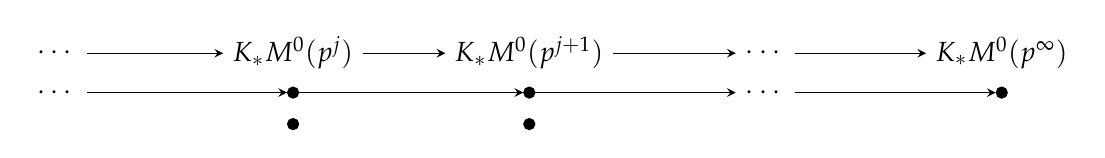
\begin{tikzpicture}[
    baseline=(current bounding box.center),
    normal line/.style={-stealth},
    node distance=3cm,
]
\node (m-1-1) {$\cdots$};
\node[right of=m-1-1] (m-1-2) {$K_* M^0(p^j)$};
\node[right of=m-1-2] (m-1-3) {$K_* M^0(p^{j+1})$};
\node[right of=m-1-3] (m-1-4) {$\cdots$};
\node[right of=m-1-4] (m-1-5) {$K_* M^0(p^\infty)$};
    \path[normal line]
        (m-1-1) edge (m-1-2)
        (m-1-2) edge (m-1-3)
        (m-1-3) edge (m-1-4)
        (m-1-4) edge (m-1-5)
;
\node[below of=m-1-1,node distance=0.5cm] (updot-1) {$\cdots$};
\node[below of=m-1-2,shape=circle,draw,node distance=0.5cm,minimum size=4pt,inner sep=0pt,fill] (updot-2) {};
\node[below of=m-1-2,shape=circle,draw,node distance=0.9cm,minimum size=4pt,inner sep=0pt,fill] (downdot-2) {};
\node[below of=m-1-3,shape=circle,draw,node distance=0.5cm,minimum size=4pt,inner sep=0pt,fill] (updot-3) {};
\node[below of=m-1-3,shape=circle,draw,node distance=0.9cm,minimum size=4pt,inner sep=0pt,fill] (downdot-3) {};
\node[below of=m-1-4,node distance=0.5cm] (updot-4) {$\cdots$};
\node[below of=m-1-5,shape=circle,draw,node distance=0.5cm,minimum size=4pt,inner sep=0pt,fill] (updot-5) {};
\path[normal line]
    (updot-1) edge (updot-2)
    (updot-2) edge (updot-3)
    (updot-3) edge (updot-4)
    (updot-4) edge (updot-5);
\end{tikzpicture}
\end{center}
\caption{``Cell diagram'' of $K_* M^0(p^\infty)$.}\label{CellDiagramFigure}
\end{figure}
This suggests a way we can modify this construction: if we insert other maps which are $K$--homology isomorphisms, then we will not harm this proof that the colimit is an invertible spectrum.  We will make use of the following results to furnish ourselves with such maps:

\begin{definition}[{\cite[Definition 1.5.3]{RavenelOrangeBook}}]
A finite spectrum $X$ is said to be of type $d$ when it is $\Gamma$--locally acyclic for all $\Gamma$ of height strictly less than $d$ and $\Gamma$--locally nontrivial for a $\Gamma$ of height exactly $d$.  (In fact, it suffices to check that acyclicity condition for any single $\Gamma$ of height $(d-1)$~\cite[Theorem 2.11]{RavenelLocalizationWRTPeriodic}.)
\end{definition}

\begin{theorem}[{Devinatz--Hopkins--Smith~\cite[Theorem 9]{HopkinsSmith}}]
A $p$--local finite spectrum $X$ is of type $d$ if and only if for $N \gg 0$ there is a map $v: \Susp^N X \to X$ which is an isomorphism in $K_\Gamma$--homology for $\Gamma$ of height $d$ and which induces the zero map in $K_\Gamma$--homology for $\Gamma$ not of height $d$.
\end{theorem}

\begin{lemma}[{Adams~\cite[Lemma 12.5]{AdamsJXIV}}]\label{AdamsSelfMaps}
The spectrum $M^0(p^{j+1})$ is type $1$ and it admits a map \[v_1^{p^j}: M^{2p^j(p-1)}(p^{j+1}) \to M^0(p^{j+1})\] which induces multiplication by $v_1^{p^j}$ in $K(1)$--homology.\footnote{Here $K(1)$ is the close cousin of $K_{\G_m}$ described in \Cref{MinimalSummands}.} Moreover, the following square commutes:
\begin{center}
\begin{tikzcd}
M^{2p^j(p-1)}(p^j) \arrow{r}{\left(v_1^{p^{j-1}}\right)^p} \arrow{d} & M^0(p^j) \arrow{d} \\
M^{2p^j(p-1)}(p^{j+1}) \arrow{r}{v_1^{p^j}} & M^0(p^{j+1}).
\end{tikzcd}
\end{center}
\end{lemma}

Selecting a $p$-adic integer $a_\infty = \sum_{j=0}^\infty c_j p^j$ with $0 \le c_j < p$, one can now construct the system \[\cdots \to M^{-|v_1| a_{j-1}}(p^j) \to M^{-|v_1| a_{j-1}}(p^{j+1}) \xrightarrow{v_1^{p^j c_j}} M^{-|v_1| a_j}(p^{j+1}) \to M^{-|v_1| a_j}(p^{j+2}) \to \cdots.\] We define $\S^{-|v_1|a_\infty}$ to be its colimit.  \Cref{HMSLines} is then sufficient to check that $\S^{-|v_1| a_\infty}$ is $\G_m$--locally invertible, but more is true:
\begin{lemma}[{\cite[Proposition 2.1]{HMS}}]\label{padicPicElements}
The above construction defines an injective continuous homomorphism of groups \[\Z_p \to \Pic(\CatOf{Spectra}_{\G_m}).\]  When $p \ge 3$ (i.e., $p \ne 2$), the cosets of its image are represented by $\S^1, \ldots, \S^{|v_1|}$.  Abstractly, there is an isomorphism \[\Pic(\CatOf{Spectra}_{\G_m}) \cong \Z_p \rtimes \Z/|v_1|. \qed\]
\end{lemma}

\begin{remark}\label{PicardGroupsWeKnow}
This is the most thorough result of this kind that we know presently.  We also know a calculation of $\Pic(\CatOf{Spectra}_{K(d)})$ for $d = 1$ at $p = 2$~\cite[Theorem 3.3]{HMS}, for $d = 2$ at $p \ge 5$~\cite[Theorem 8.1]{BehrensRevisited}, and for $d = 2$ at $p = 3$~\cite[Theorem 1.2]{GHMR}.  We have partial information for $d = 2$ and $n = 2$~\cite[pg.\ 50]{StricklandInterpolate}, and we know essentially nothing for $n \ge 3$ apart from the Hopkins--Gross analysis of the Brown--Comenetz dualizing spectrum~\cite[Theorem 6]{HopkinsGrossAnnouncement} and the analogue of \Cref{padicPicElements} using ``generalized Moore spectra''~\cite[Proposition 5.14]{HopkinsSmith},~\cite[Proposition 9.2-3]{HMS}.
\end{remark}

That $\Pic(\CatOf{Spectra}_{\G_m}) \cong \Z_p$ carries a profinite topology is not an accident; this, too, is found to be an effect internal to algebraic topology.
\begin{lemma}[{\cite[Proposition 14.3.d]{HoveyStrickland}}]
Let $F(I)$ denote the collection of $\Gamma$--local invertible spectra which become (noncanonically) isomorphic to $L_\Gamma \S^0$ after smashing with the generalized Moore spectrum $M_0(v^I)$.  The $F(I)$ form a basis of closed neighborhoods at the identity which upon linear translation endow $\Pic(\CatOf{Spectra}_\Gamma)$ with the structure of a profinite group. \qed
\end{lemma}

This computation of the Picard group pairs well with another classical calculation:
\begin{theorem}[{\cite[Theorem 1.5]{AdamsJXIV}}]\label{UnpretentiousCalculation}
There are isomorphisms \[\pi_s L_{K(1)} \S^0 \cong \begin{cases} \Z_p & \text{when $s = 0$}, \\ \Z_p / (pk) & \text{when $s = k|v_1| - 1$}, \\ 0 & \text{otherwise}. \qed \end{cases}\]
\end{theorem}

\noindent The right--hand side of this formula can be interpreted through the $p$--adic valuations of the Bernoulli numbers --- or, equivalently, through the special negative values of the Riemann $\zeta$--function: \[\mathbb N \xrightarrow{s \mapsto \zeta(1 - s} \Q \xrightarrow{\text{denom}} \Q / \Z_{(p)} \cong \Z / p^\infty.\]  Number theorists have constructed $p$--adic analytic versions of the Riemann $\zeta$--function by interpolating its special values at negative odd integers and have found such constructions to continue to hold interesting number theoretic data~\cite{Iwasawa}.  For our purposes, it is sufficient to note that the $p$--adic valuation of $\zeta^\wedge_p(1-s)$ for a $p$--adic integer $s = k|v_1| - 1$ agrees with that of $1/(pk)$ and is nonnegative otherwise, so that the formula in \Cref{UnpretentiousCalculation} needs no modification.  However, because the variables $s$ and $k$ in the above formula are linked, taking $k$ to be a general $p$--adic integer necessitates that we also take $s$ to be general $p$--adic integer as well.

\begin{corollary}[{Hopkins, see also Strickland~\cite{StricklandInterpolate}}]
Interpolating the homotopy groups $\pi_* L_{\G_m} \S^0$ using the spectra $\S^{-|v_1|a_\infty}$ constructed in \Cref{padicPicElements} agrees with the number theoretic $p$--adic interpolation of $\zeta$.
\end{corollary}
\begin{proof}
Generally, the cofiber sequence \[\S^n \xrightarrow{p^j} \S^n \to M_n(p^j) \to \S^{n+1} \xrightarrow{p^j} \S^{n+1}\] induces a short exact sequence \[0 \leftarrow (\pi_n X) [p^j] \leftarrow [M_n(p^j), X] \leftarrow (\pi_{n+1} X) / p^j \leftarrow 0,\] and the diagram
\begin{center}
\begin{tikzcd}
\S^n \arrow{r}{p^j} \arrow{d}{1} & \S^n \arrow{r} \arrow{d}{p} & M_n(p^j) \arrow{r} \arrow{d} & \S^{n+1} \arrow{r}{p^j} \arrow{d}{1} & \S^{n+1} \arrow{d}{p} \\
\S^n \arrow{r}{p^{j+1}} & \S^n \arrow{r} & M_n(p^{j+1}) \arrow{r} & \S^{n+1} \arrow{r}{p^{j+1}} & \S^{n+1}
\end{tikzcd}
\end{center}
induces the following map of short exact sequences:
\begin{center}
\begin{tikzcd}
0 & \arrow{l} (\pi_n X)[p^j] & {[M_n(p^j), X]} \arrow{l} & \arrow{l} (\pi_{n+1} X) / p^j & \arrow{l} 0 \\
0 & \arrow{l} \arrow{u}{p} (\pi_n X)[p^{j+1}] & {[M_n(p^{j+1}), X]} \arrow{l} \arrow{u} & \arrow{l} \arrow{u}{\text{quotient}} (\pi_{n+1} X) / (p^{j+1}) & \arrow{l} 0.
\end{tikzcd}
\end{center}
This map of short exact sequences interacts with the Adams $v_1$--self--map of \Cref{AdamsSelfMaps} according to the rectangular prism in \Cref{SelfMapFigure}.
\begin{sidewaysfigure}[ht]
\begin{center}
\begin{tikzcd}[column sep=-0.2cm,row sep=1.5cm]
& 0 & & (\pi_n X)[p^j] \arrow{ll} \arrow{ld} \arrow[leftarrow]{dd} & & {[M_n(p^j), X]} \arrow{ll} \arrow{ld} \arrow[leftarrow]{dd} & & (\pi_{n+1} X) / p^j \arrow{ll} \arrow{ld} \arrow[leftarrow]{dd} & & 0 \arrow{ll} \\
0 & & (\pi_{n-|v_1|p^j} X)[p^j] \arrow[leftarrow, crossing over]{rr} \arrow[red, in=182, out=2, leftarrow]{rrrrru}{\alpha_{j-1/j-1}^p} \arrow{ll} & & {[M_{n-|v_1|p^j}(p^j), X]} & & (\pi_{n-|v_1|p^j+1} X) / p^j \arrow[crossing over]{ll} & & 0 \arrow[crossing over]{ll} \\
& 0 & & (\pi_n X)[p^{j+1}] \arrow{ll} \arrow{ld} & & {[M_n(p^{j+1}), X]} \arrow{ll} \arrow{ld} & & (\pi_{n+1} X) / p^{j+1} \arrow{ll} \arrow{ld} \arrow[red, in=2, out=182]{llllld}{\alpha_{j/j}} & & 0 \arrow{ll} \\
0 & & (\pi_{n-|v_1|p^j} X)[p^{j+1}] \arrow{ll} \arrow[crossing over]{uu} & & {[M_{n-|v_1|p^j}(p^{j+1}), X]} \arrow[crossing over]{uu} \arrow{ll} & & (\pi_{n-|v_1|p^j+1} X) / p^{j+1} \arrow{ll} \arrow[crossing over]{uu} & & 0. \arrow{ll}
\end{tikzcd}
\end{center}
\caption{Interaction of Adams's $v_1$--self--maps with Moore spectra of different indices.}
\label{SelfMapFigure}
\end{sidewaysfigure}
The result follows immediately from the construction of $\S^{-|v_1| a_\infty}$.
%\todo{Actually check that this is sufficient. What about the $v_1$--self--maps?}
\end{proof}

\begin{remark}
We caution the reader that the behavior of the Picard--graded homotopy of the $\Gamma$--local sphere for $\operatorname{ht}(\Gamma) > 1$ is considerably more strangely (i.e., poorly) behaved than that of the $\G_m$--local sphere.  Hovey and Strickland prove a partial ``continuity'' result~\cite[Proposition 14.6]{HoveyStrickland} but also provide details on the remaining bad behavior~\cite[Theorem 15.1]{HoveyStrickland}.  The punchline of the bad news is as follows: take $\Gamma$ to be of height at least $2$, and define $F$ to be the set \[F := \{\lambda \in \Pic(\CatOf{Spectra}_\Gamma) : |\pi_\lambda L_{\Gamma} M^0(p)| < \infty\}.\] Then there is a nonempty open $U$ for which $U \cap F$ is Haar--negligible.  Nonetheless, all but finitely many of the standard spheres belong to $F$ --- a curious situation.
\end{remark}

\begin{remark}
Having set up some of the groundwork of chromatic homotopy theory, we pause to make a remark on the philosophy of the rest of this document.  The other homotopical context in which Picard--graded homotopy groups have taken central relevance is equivariant homotopy theory, which concerns itself with spaces and spectra with a suitable notion of a ``$G$--action'', $G$ a compact Lie group.  The notion of ``$G$--action'' turns out to be somewhat complex, and the correct notion enjoys a notion of cellular approximation, where the cells are formed as follows: for a $G$--representation $V$ we form the representation sphere $S^V$ by compactifying $V$ with a single point at $\infty$.  Cellular approximation then states that any map of $G$--spaces can be $G$--equivariantly weakly replaced by a map of ``$G$--CW--complex'', which are suitably built from the spheres $S^V$ as $V$ ranges.

The analogous construction in chromatic homotopy theory has not appeared before. Although Picard--graded phenomena in the $\Gamma$--local category have been studied, ``Picard--cellular'' constructions have escaped attention.  The primary goal of the remainder of the present work is to construct and study a certain Picard--cellular filtration of $\Gamma$--localized Eilenberg--Mac Lane spaces.
\end{remark}



\end{document}
